\documentclass[a4paper]{book}
\usepackage{a4wide}
\usepackage{makeidx}
\usepackage{fancyhdr}
\usepackage{graphicx}
\usepackage{multicol}
\usepackage{float}
\usepackage{textcomp}
\usepackage{alltt}
\usepackage{times}
\usepackage[utf8]{inputenc}
\usepackage[T2A]{fontenc}
\usepackage[czech]{babel}

\usepackage{doxygen}
\makeindex
\setcounter{tocdepth}{1}
\renewcommand{\footrulewidth}{0.4pt}
\begin{document}
\begin{titlepage}
\vspace*{7cm}
\begin{center}
{\Large Webová aplikace k projektu měření objemu řeziva Referenční příručka\\[1ex]\large 1.0 }\\
\vspace*{1cm}
{\large Generováno programem Doxygen 1.5.2}\\
\vspace*{0.5cm}
{\small Sun Sep 16 23:14:22 2007}\\
\end{center}
\end{titlepage}
\clearemptydoublepage
\pagenumbering{roman}
\tableofcontents
\clearemptydoublepage
\pagenumbering{arabic}
\chapter{Webová aplikace projektu měření objemu řeziva. }
\label{index}Tento text představuje dokumentaci k projektu měření objemu řeziva na pile.

Vzhledem k relativní jednoduchosti jsou jako výpočetní prostředky zvoleny jednočipové mikropočítače. V jejich prospěch hovoří, nízká pořizovací cena, široká dostupnost technologie, ale i to, že díky nim lze zařízení snadno rozdělit na dvě části.



První část zajišťuje obsluhu měření průměrů na katru a odeslání získaných dat do druhé části na vozíku. Měření vertikálního průměru provádí inkrementální čidlo spojené s osou motoru, který pohybuje horním přítlačným válcem nahoru a dolu. Dále je instalováno jednoduché magnetické relé, které slouží jako referenční bod. Pokaždé, když spínač sepne a průměr dv se zvětšuje, dojde k nastavení čítače vzdálenosti na přednastavenou hodnotu. Horizontální průměr bude experimentálně měřen bezkontaktní metodou s použitím jednoho zdroje světla. Nad řezaným dřevem bude umístěn halogenový světelný zdroj a pod dřevem bude měřící lišta. Na té bude řada fotodiod, které budou sloužit k měření světelné intenzity v jednotlivých bodech. Druhá část se nalézá na pojízdném vozíku. Zajišťuje obsluhu měření délky stromu, shromažďování dat, uživatelské rozhraní a komunikaci s kancelářským PC. Délka stromu se měří s využitím inkrementálního čidla. To je přiděláno na kolečko, které se odvaluje po kolejnici, po níž vozík jezdí. Uživatelské rozhraní je realizováno znakovým LCD displejem a běžnou počítačovou klávesnicí, která bude v budoucnu nahrazena průmyslovou klávesnicí. Jako výpočetní prvky byly zvoleny jednočipy Atmel. Vyznačují se nízkou cenou, slušnými výkony a lze je programovat bez dalšího příslušenství pouze prostřednictvím paralelního portu běžného PC. Pro zařízení na katru byl vybrán typ ATmega8 pro zařízení na vozíku byl zvolen typ ATmega32.\section{Odkazy}\label{index_Odkazy}
{\tt http://winavr.sourceforge.net}

{\tt http://www.mysql.com} 
\chapter{Webová aplikace k projektu měření objemu řeziva Rejstřík hierarchie tříd}
\section{Webová aplikace k projektu měření objemu řeziva Hierarchie tříd}
Zde naleznete seznam, vyjadřující vztah dědičnosti tříd. Je seřazen přibližně (ale ne úplně) podle abecedy:\begin{CompactList}
\item \contentsline{section}{kalendar}{\pageref{classkalendar}}{}
\item \contentsline{section}{nacteniZeSouboru}{\pageref{classnacteniZeSouboru}}{}
\item \contentsline{section}{Template}{\pageref{classTemplate}}{}
\begin{CompactList}
\item \contentsline{section}{CachedTemplate}{\pageref{classCachedTemplate}}{}
\end{CompactList}
\end{CompactList}

\chapter{Webová aplikace k projektu měření objemu řeziva Rejstřík datových struktur}
\section{Webová aplikace k projektu měření objemu řeziva Datové struktury}
Následující seznam obsahuje identifikace datových struktur a jejich stručné popisy:\begin{CompactList}
\item\contentsline{section}{{\bf CachedTemplate} }{\pageref{classCachedTemplate}}{}
\item\contentsline{section}{{\bf kalendar} }{\pageref{classkalendar}}{}
\item\contentsline{section}{{\bf nacteniZeSouboru} }{\pageref{classnacteniZeSouboru}}{}
\item\contentsline{section}{{\bf Template} }{\pageref{classTemplate}}{}
\end{CompactList}

\chapter{Webová aplikace k projektu měření objemu řeziva Rejstřík souborů}
\section{Webová aplikace k projektu měření objemu řeziva Seznam souborů}
Zde naleznete seznam všech souborů se stručnými popisy:\begin{CompactList}
\item\contentsline{section}{{\bf add\_\-user.php} }{\pageref{add__user_8php}}{}
\item\contentsline{section}{{\bf add\_\-zakaznik.php} }{\pageref{add__zakaznik_8php}}{}
\item\contentsline{section}{{\bf all.tmpl.php} }{\pageref{all_8tmpl_8php}}{}
\item\contentsline{section}{{\bf ceny.php} }{\pageref{ceny_8php}}{}
\item\contentsline{section}{{\bf ceny.tmpl.php} }{\pageref{ceny_8tmpl_8php}}{}
\item\contentsline{section}{{\bf config.inc.php} }{\pageref{config_8inc_8php}}{}
\item\contentsline{section}{{\bf connect\_\-info.inc.php} }{\pageref{connect__info_8inc_8php}}{}
\item\contentsline{section}{{\bf edit\_\-seznam.php} }{\pageref{edit__seznam_8php}}{}
\item\contentsline{section}{{\bf edit\_\-seznam.tmpl.php} }{\pageref{edit__seznam_8tmpl_8php}}{}
\item\contentsline{section}{{\bf edit\_\-user.php} }{\pageref{edit__user_8php}}{}
\item\contentsline{section}{{\bf edit\_\-zakaznik.php} }{\pageref{edit__zakaznik_8php}}{}
\item\contentsline{section}{{\bf edit\_\-zakaznik.tmpl.php} }{\pageref{edit__zakaznik_8tmpl_8php}}{}
\item\contentsline{section}{{\bf funkce.inc.php} }{\pageref{funkce_8inc_8php}}{}
\item\contentsline{section}{{\bf index.php} }{\pageref{index_8php}}{}
\item\contentsline{section}{{\bf kalendar.class.php} }{\pageref{kalendar_8class_8php}}{}
\item\contentsline{section}{{\bf load\_\-file.php} }{\pageref{load__file_8php}}{}
\item\contentsline{section}{{\bf load\_\-file.tmpl.php} }{\pageref{load__file_8tmpl_8php}}{}
\item\contentsline{section}{{\bf login.php} }{\pageref{login_8php}}{}
\item\contentsline{section}{{\bf menu.inc.php} }{\pageref{menu_8inc_8php}}{}
\item\contentsline{section}{{\bf menu\_\-root.inc.php} (Tlačítka menu, která jsou načtena při přihlášení roota )}{\pageref{menu__root_8inc_8php}}{}
\item\contentsline{section}{{\bf mysql.inc.php} }{\pageref{mysql_8inc_8php}}{}
\item\contentsline{section}{{\bf mysqli.inc.php} }{\pageref{mysqli_8inc_8php}}{}
\item\contentsline{section}{{\bf nacteniZeSouboru.class.php} }{\pageref{nacteniZeSouboru_8class_8php}}{}
\item\contentsline{section}{{\bf new\_\-seznam.php} }{\pageref{new__seznam_8php}}{}
\item\contentsline{section}{{\bf nova\_\-mereni.php} }{\pageref{nova__mereni_8php}}{}
\item\contentsline{section}{{\bf nove\_\-mereni.tmpl.php} }{\pageref{nove__mereni_8tmpl_8php}}{}
\item\contentsline{section}{{\bf ok.php} }{\pageref{ok_8php}}{}
\item\contentsline{section}{{\bf ok.tmpl.php} }{\pageref{ok_8tmpl_8php}}{}
\item\contentsline{section}{{\bf print.tmpl.php} }{\pageref{print_8tmpl_8php}}{}
\item\contentsline{section}{{\bf safe\_\-ip.inc.php} }{\pageref{safe__ip_8inc_8php}}{}
\item\contentsline{section}{{\bf session\_\-close.php} }{\pageref{session__close_8php}}{}
\item\contentsline{section}{{\bf seznam.php} }{\pageref{seznam_8php}}{}
\item\contentsline{section}{{\bf seznam.tmpl.php} }{\pageref{seznam_8tmpl_8php}}{}
\item\contentsline{section}{{\bf seznamy.php} (Soubor zajišťuje vypisování zakázek zákazníků )}{\pageref{seznamy_8php}}{}
\item\contentsline{section}{{\bf seznamy.tmpl.php} }{\pageref{seznamy_8tmpl_8php}}{}
\item\contentsline{section}{{\bf stat.tmpl.php} }{\pageref{stat_8tmpl_8php}}{}
\item\contentsline{section}{{\bf template.class.php} }{\pageref{template_8class_8php}}{}
\item\contentsline{section}{{\bf user.tmpl.php} }{\pageref{user_8tmpl_8php}}{}
\item\contentsline{section}{{\bf users.php} }{\pageref{users_8php}}{}
\item\contentsline{section}{{\bf users.tmpl.php} }{\pageref{users_8tmpl_8php}}{}
\item\contentsline{section}{{\bf volni\_\-zakaznici\_\-mereni.tmpl.php} }{\pageref{volni__zakaznici__mereni_8tmpl_8php}}{}
\item\contentsline{section}{{\bf zakazky.php} }{\pageref{zakazky_8php}}{}
\item\contentsline{section}{{\bf zakazky.tmpl.php} }{\pageref{zakazky_8tmpl_8php}}{}
\item\contentsline{section}{{\bf zakaznici.tmpl.php} }{\pageref{zakaznici_8tmpl_8php}}{}
\item\contentsline{section}{{\bf zakaznici\_\-all.tmpl.php} }{\pageref{zakaznici__all_8tmpl_8php}}{}
\item\contentsline{section}{{\bf zakaznici\_\-mereni.php} }{\pageref{zakaznici__mereni_8php}}{}
\item\contentsline{section}{{\bf zakaznici\_\-mereni.tmpl.php} }{\pageref{zakaznici__mereni_8tmpl_8php}}{}
\item\contentsline{section}{{\bf zakaznik.php} }{\pageref{zakaznik_8php}}{}
\item\contentsline{section}{{\bf zakaznik.tmpl.php} }{\pageref{zakaznik_8tmpl_8php}}{}
\item\contentsline{section}{{\bf zakaznik\_\-form.tmpl.php} }{\pageref{zakaznik__form_8tmpl_8php}}{}
\item\contentsline{section}{{\bf zakaznik\_\-seznam.php} }{\pageref{zakaznik__seznam_8php}}{}
\item\contentsline{section}{{\bf zakaznik\_\-seznam.tmpl.php} }{\pageref{zakaznik__seznam_8tmpl_8php}}{}
\item\contentsline{section}{{\bf zarad.php} }{\pageref{zarad_8php}}{}
\item\contentsline{section}{{\bf zarad.tmpl.php} }{\pageref{zarad_8tmpl_8php}}{}
\end{CompactList}

\chapter{Webová aplikace k projektu měření objemu řeziva Rejstřík stránek}
\section{Webová aplikace k projektu měření objemu řeziva Ostatní stránky}
Následující seznam odkazuje na další stránky projektu:\begin{CompactList}
\item \contentsline{section}{Manu�l k webov� aplikaci}{\pageref{web_manual}}{}

\item \contentsline{section}{Seznam plánovaných úprav}{\pageref{todo}}{}

\end{CompactList}

\chapter{Webová aplikace k projektu měření objemu řeziva Dokumentace datových struktur}
\section{Dokumentace třídy CachedTemplate}
\label{classCachedTemplate}\index{CachedTemplate@{CachedTemplate}}
Diagram dědičnosti pro třídu CachedTemplate:\begin{figure}[H]
\begin{center}
\leavevmode
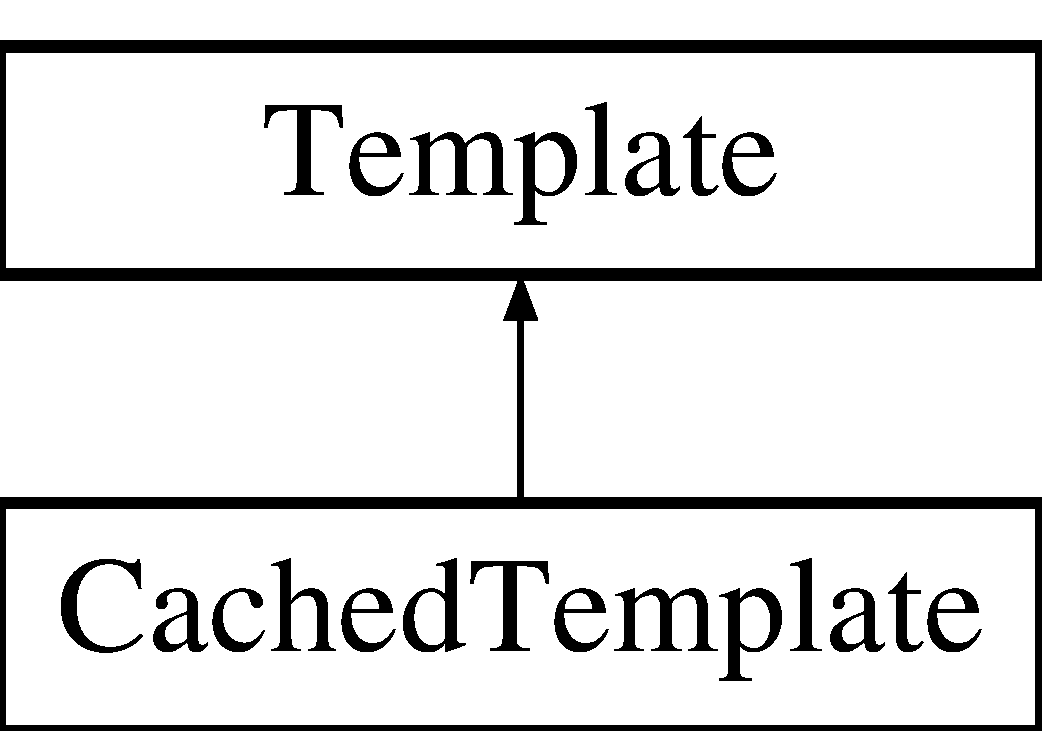
\includegraphics[height=2cm]{classCachedTemplate}
\end{center}
\end{figure}
\subsection*{Veřejné metody}
\begin{CompactItemize}
\item 
{\bf CachedTemplate} (\$cache\_\-id=null, \$expire=900)
\item 
{\bf is\_\-cached} ()
\item 
{\bf fetch\_\-cache} (\$file)
\end{CompactItemize}
\subsection*{Datové položky}
\begin{CompactItemize}
\item 
{\bf \$cache\_\-id}
\item 
{\bf \$expire}
\item 
{\bf \$cached}
\end{CompactItemize}


\subsection{Detailní popis}
An extension to \doxyref{Template}{s.}{classTemplate} that provides automatic caching of template contents. 



\subsection{Dokumentace k metodám}
\index{CachedTemplate@{CachedTemplate}!CachedTemplate@{CachedTemplate}}
\index{CachedTemplate@{CachedTemplate}!CachedTemplate@{CachedTemplate}}
\subsubsection{\setlength{\rightskip}{0pt plus 5cm}CachedTemplate::CachedTemplate (\$ {\em cache\_\-id} = {\tt null}, \$ {\em expire} = {\tt 900})}\label{classCachedTemplate_1faa0e63bb5473509022fe8f415fc560}


Constructor.

\begin{Desc}
\item[Parametry:]
\begin{description}
\item[{\em \$cache\_\-id}]string unique cache identifier \item[{\em \$expire}]int number of seconds the cache will live \end{description}
\end{Desc}
\index{CachedTemplate@{CachedTemplate}!is_cached@{is\_\-cached}}
\index{is_cached@{is\_\-cached}!CachedTemplate@{CachedTemplate}}
\subsubsection{\setlength{\rightskip}{0pt plus 5cm}CachedTemplate::is\_\-cached ()}\label{classCachedTemplate_34ae05b638aad2a22e677c6845f4ef43}


Test to see whether the currently loaded cache\_\-id has a valid corrosponding cache file. 

Cache the results of this \doxyref{is\_\-cached()}{s.}{classCachedTemplate_34ae05b638aad2a22e677c6845f4ef43} call. Why? So we don't have to double the overhead for each template. If we didn't cache, it would be hitting the file system twice as much (file\_\-exists() \& filemtime() [twice each]). \index{CachedTemplate@{CachedTemplate}!fetch_cache@{fetch\_\-cache}}
\index{fetch_cache@{fetch\_\-cache}!CachedTemplate@{CachedTemplate}}
\subsubsection{\setlength{\rightskip}{0pt plus 5cm}CachedTemplate::fetch\_\-cache (\$ {\em file})}\label{classCachedTemplate_db9de9d3ea96a25c895876df27260722}


This function returns a cached copy of a template (if it exists), otherwise, it parses it as normal and caches the content.

\begin{Desc}
\item[Parametry:]
\begin{description}
\item[{\em \$file}]string the template file \end{description}
\end{Desc}


\subsection{Dokumentace k položkám}
\index{CachedTemplate@{CachedTemplate}!$cache_id@{\$cache\_\-id}}
\index{$cache_id@{\$cache\_\-id}!CachedTemplate@{CachedTemplate}}
\subsubsection{\setlength{\rightskip}{0pt plus 5cm}CachedTemplate::\$cache\_\-id}\label{classCachedTemplate_1862568621acd4c78e325b045811d091}


\index{CachedTemplate@{CachedTemplate}!$expire@{\$expire}}
\index{$expire@{\$expire}!CachedTemplate@{CachedTemplate}}
\subsubsection{\setlength{\rightskip}{0pt plus 5cm}CachedTemplate::\$expire}\label{classCachedTemplate_e1fa8b2f2da35d463b69047643c4f1f2}


\index{CachedTemplate@{CachedTemplate}!$cached@{\$cached}}
\index{$cached@{\$cached}!CachedTemplate@{CachedTemplate}}
\subsubsection{\setlength{\rightskip}{0pt plus 5cm}CachedTemplate::\$cached}\label{classCachedTemplate_2e6fab9f815c00587bd37d0fde91b7c6}




Dokumentace pro tuto třídu byla generována z následujícího souboru:\begin{CompactItemize}
\item 
{\bf template.class.php}\end{CompactItemize}

\section{Dokumentace třídy kalendar}
\label{classkalendar}\index{kalendar@{kalendar}}
\subsection*{Veřejné metody}
\begin{CompactItemize}
\item 
{\bf pocetDnu} (\$mesic, \$rok)
\item 
{\bf prvniDen} (\$mesic, \$rok)
\item 
{\bf bunka} (\$radek, \$sloupec, \$PrvniDen, \$PocetDnu)
\item 
{\bf vypis} (\$mesic, \$rok)
\end{CompactItemize}


\subsection{Detailní popis}
\begin{Desc}
\item[Id]\doxyref{kalendar.class.php}{s.}{kalendar_8class_8php} 77 2007-08-13 16:43:56Z Mira \end{Desc}




\subsection{Dokumentace k metodám}
\index{kalendar@{kalendar}!pocetDnu@{pocetDnu}}
\index{pocetDnu@{pocetDnu}!kalendar@{kalendar}}
\subsubsection{\setlength{\rightskip}{0pt plus 5cm}kalendar::pocetDnu (\$ {\em mesic}, \$ {\em rok})}\label{classkalendar_c1fd0fdea3f8f24c5140867310e63334}


Funkce vrací počet dnů v měsíci. \index{kalendar@{kalendar}!prvniDen@{prvniDen}}
\index{prvniDen@{prvniDen}!kalendar@{kalendar}}
\subsubsection{\setlength{\rightskip}{0pt plus 5cm}kalendar::prvniDen (\$ {\em mesic}, \$ {\em rok})}\label{classkalendar_b482f153ddb104e81fd5fb7b2b24c542}


Funkce vrací číslo prvního dne v týdnu. \index{kalendar@{kalendar}!bunka@{bunka}}
\index{bunka@{bunka}!kalendar@{kalendar}}
\subsubsection{\setlength{\rightskip}{0pt plus 5cm}kalendar::bunka (\$ {\em radek}, \$ {\em sloupec}, \$ {\em PrvniDen}, \$ {\em PocetDnu})}\label{classkalendar_05c62a04cf86c5e81f15f86b36c1386e}


\index{kalendar@{kalendar}!vypis@{vypis}}
\index{vypis@{vypis}!kalendar@{kalendar}}
\subsubsection{\setlength{\rightskip}{0pt plus 5cm}kalendar::vypis (\$ {\em mesic}, \$ {\em rok})}\label{classkalendar_6bb64912e1b8f7e69f96092f45d34ef3}




Dokumentace pro tuto třídu byla generována z následujícího souboru:\begin{CompactItemize}
\item 
{\bf kalendar.class.php}\end{CompactItemize}

\section{Dokumentace třídy nacteniZeSouboru}
\label{classnacteniZeSouboru}\index{nacteniZeSouboru@{nacteniZeSouboru}}


Dokumentace pro tuto třídu byla generována z následujícího souboru:\begin{CompactItemize}
\item 
{\bf nacteniZeSouboru.class.php}\end{CompactItemize}

\section{Dokumentace třídy Template}
\label{classTemplate}\index{Template@{Template}}
Diagram dědičnosti pro třídu Template:\begin{figure}[H]
\begin{center}
\leavevmode
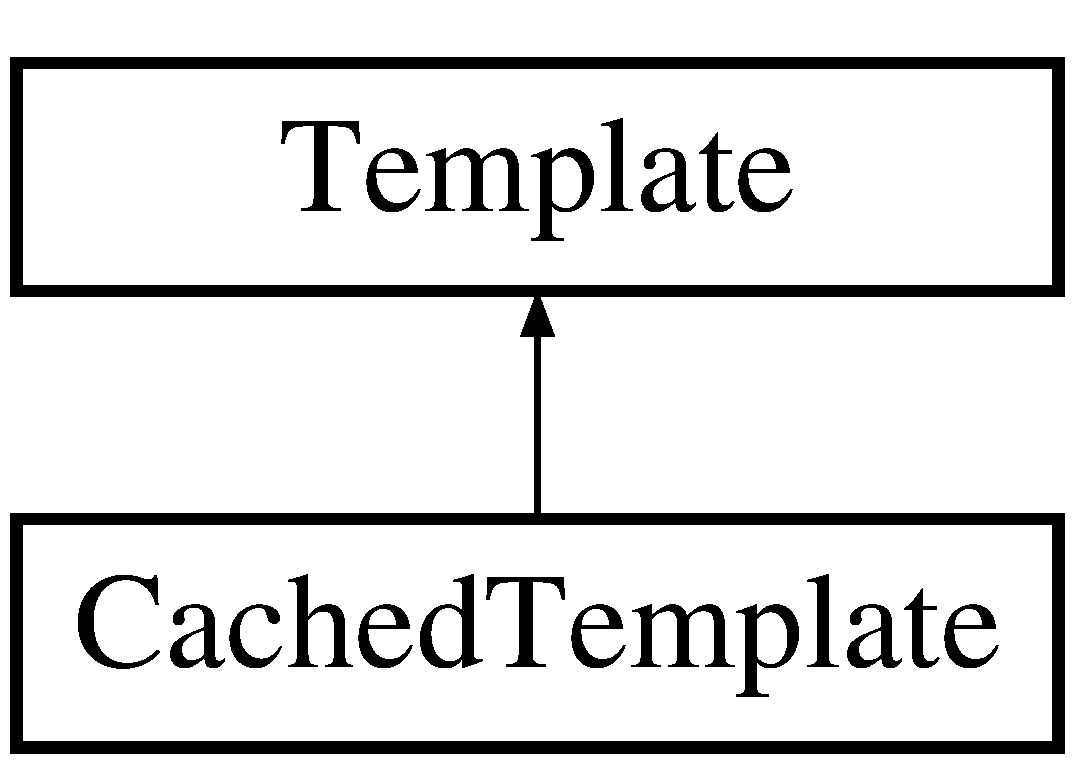
\includegraphics[height=2cm]{classTemplate}
\end{center}
\end{figure}
\subsection*{Veřejné metody}
\begin{CompactItemize}
\item 
{\bf Template} (\$file=null)
\begin{CompactList}\small\item\em Holds all the template variables. \item\end{CompactList}\item 
{\bf set} (\$name, \$value)
\item 
{\bf fetch} (\$file=null)
\end{CompactItemize}
\subsection*{Datové položky}
\begin{CompactItemize}
\item 
{\bf \$vars}
\end{CompactItemize}


\subsection{Dokumentace k metodám}
\index{Template@{Template}!Template@{Template}}
\index{Template@{Template}!Template@{Template}}
\subsubsection{\setlength{\rightskip}{0pt plus 5cm}Template::Template (\$ {\em file} = {\tt null})}\label{classTemplate_4b9d12f1073d2c9a7e5608f0034810d4}


Holds all the template variables. 

Constructor

\begin{Desc}
\item[Parametry:]
\begin{description}
\item[{\em \$file}]string the file name you want to load \end{description}
\end{Desc}
\index{Template@{Template}!set@{set}}
\index{set@{set}!Template@{Template}}
\subsubsection{\setlength{\rightskip}{0pt plus 5cm}Template::set (\$ {\em name}, \$ {\em value})}\label{classTemplate_b1c9904c0a6f4242cc5e4392b63a241d}


Set a template variable. \index{Template@{Template}!fetch@{fetch}}
\index{fetch@{fetch}!Template@{Template}}
\subsubsection{\setlength{\rightskip}{0pt plus 5cm}Template::fetch (\$ {\em file} = {\tt null})}\label{classTemplate_9d4da74dc991725da1603fe9ea9380c9}


Open, parse, and return the template file.

\begin{Desc}
\item[Parametry:]
\begin{description}
\item[{\em \$file}]string the template file name \end{description}
\end{Desc}


\subsection{Dokumentace k položkám}
\index{Template@{Template}!$vars@{\$vars}}
\index{$vars@{\$vars}!Template@{Template}}
\subsubsection{\setlength{\rightskip}{0pt plus 5cm}Template::\$vars}\label{classTemplate_4ea3fb3e81eb30dae82ef45493d84bf3}




Dokumentace pro tuto třídu byla generována z následujícího souboru:\begin{CompactItemize}
\item 
{\bf template.class.php}\end{CompactItemize}

\chapter{Webová aplikace k projektu měření objemu řeziva Dokumentace souborů}
\section{Dokumentace souboru add\_\-user.php}
\label{add__user_8php}\index{add_user.php@{add\_\-user.php}}
\subsection*{Proměnné}
\begin{CompactItemize}
\item 
{\bf \$link} = connect\_\-db()
\item 
{\bf \$all} = \& new {\bf Template}('./tmpl/all.tmpl.php')
\item 
{\bf \$body} = \& new {\bf Template}('./tmpl/user.tmpl.php')
\item 
{\bf \$BudemeZobrazovat} = true
\item 
{\bf \$echo} = null
\end{CompactItemize}


\subsection{Detailní popis}
\$file\$ \$File\$ Soubor zajišťuje přidání nového uživatele. 

\subsection{Dokumentace proměnných}
\index{add_user.php@{add\_\-user.php}!$all@{\$all}}
\index{$all@{\$all}!add_user.php@{add\_\-user.php}}
\subsubsection{\setlength{\rightskip}{0pt plus 5cm}\$all = \& new {\bf Template}('./tmpl/all.tmpl.php')}\label{add__user_8php_3c74ea9d2348c9aba28d36e692bef2d2}


\index{add_user.php@{add\_\-user.php}!$body@{\$body}}
\index{$body@{\$body}!add_user.php@{add\_\-user.php}}
\subsubsection{\setlength{\rightskip}{0pt plus 5cm}\$body = \& new {\bf Template}('./tmpl/user.tmpl.php')}\label{add__user_8php_26b9f9373f7bb79dfcf8a86dff086b45}


\index{add_user.php@{add\_\-user.php}!$BudemeZobrazovat@{\$BudemeZobrazovat}}
\index{$BudemeZobrazovat@{\$BudemeZobrazovat}!add_user.php@{add\_\-user.php}}
\subsubsection{\setlength{\rightskip}{0pt plus 5cm}\$BudemeZobrazovat = true}\label{add__user_8php_7257dc22059027fb436043d05c4adc71}


\index{add_user.php@{add\_\-user.php}!$echo@{\$echo}}
\index{$echo@{\$echo}!add_user.php@{add\_\-user.php}}
\subsubsection{\setlength{\rightskip}{0pt plus 5cm}\$echo = null}\label{add__user_8php_76dbdd763137ce9b516dc94d3a16fe60}


\index{add_user.php@{add\_\-user.php}!$link@{\$link}}
\index{$link@{\$link}!add_user.php@{add\_\-user.php}}
\subsubsection{\setlength{\rightskip}{0pt plus 5cm}\$link = connect\_\-db()}\label{add__user_8php_5d346e31b75d916e3bac9cb193bfc97f}



\section{Dokumentace souboru add\_\-zakaznik.php}
\label{add__zakaznik_8php}\index{add_zakaznik.php@{add\_\-zakaznik.php}}
\subsection*{Proměnné}
\begin{CompactItemize}
\item 
{\bf \$BudemeZobrazovat} = true
\item 
{\bf \$check} = insertZakaznik(\$\_\-POST,\$link)
\item 
{\bf endif}
\item 
{\bf \$all} = \& new {\bf Template}('./tmpl/all.tmpl.php')
\item 
{\bf \$body} = \& new {\bf Template}('./tmpl/edit\_\-zakaznik.tmpl.php')
\end{CompactItemize}


\subsection{Detailní popis}
Skript zajišťuje přidávání zákazníků. 

\subsection{Dokumentace proměnných}
\index{add_zakaznik.php@{add\_\-zakaznik.php}!$all@{\$all}}
\index{$all@{\$all}!add_zakaznik.php@{add\_\-zakaznik.php}}
\subsubsection{\setlength{\rightskip}{0pt plus 5cm}\$all = \& new {\bf Template}('./tmpl/all.tmpl.php')}\label{add__zakaznik_8php_3c74ea9d2348c9aba28d36e692bef2d2}


\index{add_zakaznik.php@{add\_\-zakaznik.php}!$body@{\$body}}
\index{$body@{\$body}!add_zakaznik.php@{add\_\-zakaznik.php}}
\subsubsection{\setlength{\rightskip}{0pt plus 5cm}\$body = \& new {\bf Template}('./tmpl/edit\_\-zakaznik.tmpl.php')}\label{add__zakaznik_8php_26b9f9373f7bb79dfcf8a86dff086b45}


\index{add_zakaznik.php@{add\_\-zakaznik.php}!$BudemeZobrazovat@{\$BudemeZobrazovat}}
\index{$BudemeZobrazovat@{\$BudemeZobrazovat}!add_zakaznik.php@{add\_\-zakaznik.php}}
\subsubsection{\setlength{\rightskip}{0pt plus 5cm}\$BudemeZobrazovat = true}\label{add__zakaznik_8php_7257dc22059027fb436043d05c4adc71}


\index{add_zakaznik.php@{add\_\-zakaznik.php}!$check@{\$check}}
\index{$check@{\$check}!add_zakaznik.php@{add\_\-zakaznik.php}}
\subsubsection{\setlength{\rightskip}{0pt plus 5cm}\$check = insertZakaznik(\$\_\-POST,\$link)}\label{add__zakaznik_8php_830cf70d25fefacddcf4c6bc3fd7a0e0}


\index{add_zakaznik.php@{add\_\-zakaznik.php}!endif@{endif}}
\index{endif@{endif}!add_zakaznik.php@{add\_\-zakaznik.php}}
\subsubsection{\setlength{\rightskip}{0pt plus 5cm}{\bf endif}}\label{add__zakaznik_8php_82cd33ca97ff99f2fcc5e9c81d65251b}



\section{Dokumentace souboru all.tmpl.php}
\label{all_8tmpl_8php}\index{all.tmpl.php@{all.tmpl.php}}
\subsection*{Proměnné}
\begin{CompactItemize}
\item 
else {\bf \_\-\_\-pad0\_\-\_\-}
\item 
{\bf charset}
\item 
{\bf endif}
\end{CompactItemize}


\subsection{Dokumentace proměnných}
\index{all.tmpl.php@{all.tmpl.php}!__pad0__@{\_\-\_\-pad0\_\-\_\-}}
\index{__pad0__@{\_\-\_\-pad0\_\-\_\-}!all.tmpl.php@{all.tmpl.php}}
\subsubsection{\setlength{\rightskip}{0pt plus 5cm}else {\bf \_\-\_\-pad0\_\-\_\-}}\label{all_8tmpl_8php_8e01dcc96c43199448ee66f7c2ae8ea6}


\index{all.tmpl.php@{all.tmpl.php}!charset@{charset}}
\index{charset@{charset}!all.tmpl.php@{all.tmpl.php}}
\subsubsection{\setlength{\rightskip}{0pt plus 5cm}{\bf charset}}\label{all_8tmpl_8php_8bd4accafd4e712317ed9a471738a971}


\textbf{Initializer:}

\begin{Code}\begin{verbatim}utf-8">
    <title> Dřevo </title>
    <link rel="stylesheet" type="text/css" href="style.css">
    </head>
    <body>
    <div id="head">
    <div id="headLeft">
    
    </div>
    <div id="headMain">
    <h1><?php echo $nadpis;
      if (!empty($nadpis2)){
        echo "<font size=\"4\"> - $nadpis2</font>"
\end{verbatim}
\end{Code}
\index{all.tmpl.php@{all.tmpl.php}!endif@{endif}}
\index{endif@{endif}!all.tmpl.php@{all.tmpl.php}}
\subsubsection{\setlength{\rightskip}{0pt plus 5cm}{\bf endif}}\label{all_8tmpl_8php_82cd33ca97ff99f2fcc5e9c81d65251b}



\section{Dokumentace souboru ceny.php}
\label{ceny_8php}\index{ceny.php@{ceny.php}}
\subsection*{Proměnné}
\begin{CompactItemize}
\item 
{\bf \$link} = connect\_\-db()
\item 
{\bf \$all} = \& new {\bf Template}('./tmpl/all.tmpl.php')
\item 
{\bf \$body} = \& new {\bf Template}('./tmpl/ceny.tmpl.php')
\item 
{\bf \$zdruhy} = druhy\_\-dreva(\$link)
\item 
{\bf \$ceny} = getCeny(\$link)
\end{CompactItemize}


\subsection{Detailní popis}
Soubor zajišťuje editaci cen. 

\subsection{Dokumentace proměnných}
\index{ceny.php@{ceny.php}!$all@{\$all}}
\index{$all@{\$all}!ceny.php@{ceny.php}}
\subsubsection{\setlength{\rightskip}{0pt plus 5cm}\$all = \& new {\bf Template}('./tmpl/all.tmpl.php')}\label{ceny_8php_3c74ea9d2348c9aba28d36e692bef2d2}


\index{ceny.php@{ceny.php}!$body@{\$body}}
\index{$body@{\$body}!ceny.php@{ceny.php}}
\subsubsection{\setlength{\rightskip}{0pt plus 5cm}\$body = \& new {\bf Template}('./tmpl/ceny.tmpl.php')}\label{ceny_8php_26b9f9373f7bb79dfcf8a86dff086b45}


\index{ceny.php@{ceny.php}!$ceny@{\$ceny}}
\index{$ceny@{\$ceny}!ceny.php@{ceny.php}}
\subsubsection{\setlength{\rightskip}{0pt plus 5cm}\$ceny = getCeny(\$link)}\label{ceny_8php_22c2c5c2c686d4be1f43b067588d790a}


\index{ceny.php@{ceny.php}!$link@{\$link}}
\index{$link@{\$link}!ceny.php@{ceny.php}}
\subsubsection{\setlength{\rightskip}{0pt plus 5cm}\$link = connect\_\-db()}\label{ceny_8php_5d346e31b75d916e3bac9cb193bfc97f}


\index{ceny.php@{ceny.php}!$zdruhy@{\$zdruhy}}
\index{$zdruhy@{\$zdruhy}!ceny.php@{ceny.php}}
\subsubsection{\setlength{\rightskip}{0pt plus 5cm}\$zdruhy = druhy\_\-dreva(\$link)}\label{ceny_8php_2f4727ea869082ec91e88aa9c5116231}



\section{Dokumentace souboru ceny.tmpl.php}
\label{ceny_8tmpl_8php}\index{ceny.tmpl.php@{ceny.tmpl.php}}

\section{Dokumentace souboru config.inc.php}
\label{config_8inc_8php}\index{config.inc.php@{config.inc.php}}
\subsection*{Proměnné}
\begin{CompactItemize}
\item 
{\bf \$confDalsiZpracovani} = true
\item 
{\bf \$confPodrobnyTisk} = true
\end{CompactItemize}


\subsection{Dokumentace proměnných}
\index{config.inc.php@{config.inc.php}!$confDalsiZpracovani@{\$confDalsiZpracovani}}
\index{$confDalsiZpracovani@{\$confDalsiZpracovani}!config.inc.php@{config.inc.php}}
\subsubsection{\setlength{\rightskip}{0pt plus 5cm}\$confDalsiZpracovani = true}\label{config_8inc_8php_330938b4e28d2d4f01d33c9cc6fa97f7}


\index{config.inc.php@{config.inc.php}!$confPodrobnyTisk@{\$confPodrobnyTisk}}
\index{$confPodrobnyTisk@{\$confPodrobnyTisk}!config.inc.php@{config.inc.php}}
\subsubsection{\setlength{\rightskip}{0pt plus 5cm}\$confPodrobnyTisk = true}\label{config_8inc_8php_0edd9c4b0aca24544068668305c9c7ad}



\section{Dokumentace souboru connect\_\-info.inc.php}
\label{connect__info_8inc_8php}\index{connect_info.inc.php@{connect\_\-info.inc.php}}
\subsection*{Výčty}
\begin{CompactItemize}
\item 
enum {\bf SQL\_\-DBNAME} 
\item 
enum {\bf SQL\_\-USERNAME} 
\item 
enum {\bf SQL\_\-PASSWORD} 
\item 
enum {\bf MD5\_\-PASSWORD} 
\end{CompactItemize}


\subsection{Dokumentace výčtových typů}
\index{connect_info.inc.php@{connect\_\-info.inc.php}!MD5_PASSWORD@{MD5\_\-PASSWORD}}
\index{MD5_PASSWORD@{MD5\_\-PASSWORD}!connect_info.inc.php@{connect\_\-info.inc.php}}
\subsubsection{\setlength{\rightskip}{0pt plus 5cm}enum {\bf MD5\_\-PASSWORD}}\label{connect__info_8inc_8php_ba364789fbfb101a2903d12c350cca9b}


\index{connect_info.inc.php@{connect\_\-info.inc.php}!SQL_DBNAME@{SQL\_\-DBNAME}}
\index{SQL_DBNAME@{SQL\_\-DBNAME}!connect_info.inc.php@{connect\_\-info.inc.php}}
\subsubsection{\setlength{\rightskip}{0pt plus 5cm}enum {\bf SQL\_\-DBNAME}}\label{connect__info_8inc_8php_3019042af05faafacd4763bc0cc369e8}


\index{connect_info.inc.php@{connect\_\-info.inc.php}!SQL_PASSWORD@{SQL\_\-PASSWORD}}
\index{SQL_PASSWORD@{SQL\_\-PASSWORD}!connect_info.inc.php@{connect\_\-info.inc.php}}
\subsubsection{\setlength{\rightskip}{0pt plus 5cm}enum {\bf SQL\_\-PASSWORD}}\label{connect__info_8inc_8php_585bc5fada5c786b8b2d9d27ef7b9762}


\index{connect_info.inc.php@{connect\_\-info.inc.php}!SQL_USERNAME@{SQL\_\-USERNAME}}
\index{SQL_USERNAME@{SQL\_\-USERNAME}!connect_info.inc.php@{connect\_\-info.inc.php}}
\subsubsection{\setlength{\rightskip}{0pt plus 5cm}enum {\bf SQL\_\-USERNAME}}\label{connect__info_8inc_8php_8e3d26fa8079682aa02526a592a9851f}



\section{Dokumentace souboru doc.txt}
\label{doc_8txt}\index{doc.txt@{doc.txt}}

\section{Dokumentace souboru edit\_\-seznam.php}
\label{edit__seznam_8php}\index{edit_seznam.php@{edit\_\-seznam.php}}
\subsection*{Proměnné}
\begin{CompactItemize}
\item 
{\bf \$link} = connect\_\-db()
\item 
{\bf \$all} = \& new {\bf Template}('./tmpl/all.tmpl.php')
\item 
{\bf \$body} = \& new {\bf Template}('./tmpl/edit\_\-seznam.tmpl.php')
\item 
{\bf \$tisk} = \& new {\bf Template}('./tmpl/seznam.tmpl.php')
\item 
{\bf \$novy} = \& new {\bf Template}('./tmpl/nove\_\-mereni.tmpl.php')
\item 
{\bf \$chybovaHlaska} = false
\item 
{\bf \$chybovaHlaskaCena} = false
\item 
{\bf \$ceny} = parametry\_\-seznamu(\$\_\-GET[\char`\"{}id\char`\"{}],\$link)
\item 
{\bf \$nove\_\-mer} = null
\item 
{\bf \$zaznam} [\char`\"{}Cena\_\-m3\char`\"{}] = cena\_\-strom\_\-m3 (\$zaznam,\$ceny)
\item 
{\bf \$zaznamy} [\$key] = \$zaznam
\item 
{\bf \$zdruhy} = druhy\_\-dreva(\$link)
\item 
{\bf \$dalsi\_\-zpracovani} = dalsi\_\-zpracovani(\$link)
\end{CompactItemize}


\subsection{Detailní popis}
Soubor zajišťuje editaci zakázky. 

\subsection{Dokumentace proměnných}
\index{edit_seznam.php@{edit\_\-seznam.php}!$all@{\$all}}
\index{$all@{\$all}!edit_seznam.php@{edit\_\-seznam.php}}
\subsubsection{\setlength{\rightskip}{0pt plus 5cm}\$all = \& new {\bf Template}('./tmpl/all.tmpl.php')}\label{edit__seznam_8php_3c74ea9d2348c9aba28d36e692bef2d2}


\index{edit_seznam.php@{edit\_\-seznam.php}!$body@{\$body}}
\index{$body@{\$body}!edit_seznam.php@{edit\_\-seznam.php}}
\subsubsection{\setlength{\rightskip}{0pt plus 5cm}\$body = \& new {\bf Template}('./tmpl/edit\_\-seznam.tmpl.php')}\label{edit__seznam_8php_26b9f9373f7bb79dfcf8a86dff086b45}


\index{edit_seznam.php@{edit\_\-seznam.php}!$ceny@{\$ceny}}
\index{$ceny@{\$ceny}!edit_seznam.php@{edit\_\-seznam.php}}
\subsubsection{\setlength{\rightskip}{0pt plus 5cm}\$ceny = parametry\_\-seznamu(\$\_\-GET[\char`\"{}id\char`\"{}],\$link)}\label{edit__seznam_8php_22c2c5c2c686d4be1f43b067588d790a}


\index{edit_seznam.php@{edit\_\-seznam.php}!$chybovaHlaska@{\$chybovaHlaska}}
\index{$chybovaHlaska@{\$chybovaHlaska}!edit_seznam.php@{edit\_\-seznam.php}}
\subsubsection{\setlength{\rightskip}{0pt plus 5cm}\$chybovaHlaska = false}\label{edit__seznam_8php_3c37b063b89ad1a467767a3d915a3c41}


\index{edit_seznam.php@{edit\_\-seznam.php}!$chybovaHlaskaCena@{\$chybovaHlaskaCena}}
\index{$chybovaHlaskaCena@{\$chybovaHlaskaCena}!edit_seznam.php@{edit\_\-seznam.php}}
\subsubsection{\setlength{\rightskip}{0pt plus 5cm}\$chybovaHlaskaCena = false}\label{edit__seznam_8php_78baee63a6db53573ed50117fe41fb25}


\index{edit_seznam.php@{edit\_\-seznam.php}!$dalsi_zpracovani@{\$dalsi\_\-zpracovani}}
\index{$dalsi_zpracovani@{\$dalsi\_\-zpracovani}!edit_seznam.php@{edit\_\-seznam.php}}
\subsubsection{\setlength{\rightskip}{0pt plus 5cm}\$dalsi\_\-zpracovani = dalsi\_\-zpracovani(\$link)}\label{edit__seznam_8php_4e38bd4e6c20b5e662f40ebdde8dad2b}


\index{edit_seznam.php@{edit\_\-seznam.php}!$link@{\$link}}
\index{$link@{\$link}!edit_seznam.php@{edit\_\-seznam.php}}
\subsubsection{\setlength{\rightskip}{0pt plus 5cm}\$link = connect\_\-db()}\label{edit__seznam_8php_5d346e31b75d916e3bac9cb193bfc97f}


\index{edit_seznam.php@{edit\_\-seznam.php}!$nove_mer@{\$nove\_\-mer}}
\index{$nove_mer@{\$nove\_\-mer}!edit_seznam.php@{edit\_\-seznam.php}}
\subsubsection{\setlength{\rightskip}{0pt plus 5cm}\$nove\_\-mer = null}\label{edit__seznam_8php_556d395e43784391881a80244efd7788}


\index{edit_seznam.php@{edit\_\-seznam.php}!$novy@{\$novy}}
\index{$novy@{\$novy}!edit_seznam.php@{edit\_\-seznam.php}}
\subsubsection{\setlength{\rightskip}{0pt plus 5cm}\$novy = \& new {\bf Template}('./tmpl/nove\_\-mereni.tmpl.php')}\label{edit__seznam_8php_0a14f7b921f1c1d02ff8b900d2618236}


\index{edit_seznam.php@{edit\_\-seznam.php}!$tisk@{\$tisk}}
\index{$tisk@{\$tisk}!edit_seznam.php@{edit\_\-seznam.php}}
\subsubsection{\setlength{\rightskip}{0pt plus 5cm}\$tisk = \& new {\bf Template}('./tmpl/seznam.tmpl.php')}\label{edit__seznam_8php_f75bdb3629c27f871b739f7947703e43}


\index{edit_seznam.php@{edit\_\-seznam.php}!$zaznam@{\$zaznam}}
\index{$zaznam@{\$zaznam}!edit_seznam.php@{edit\_\-seznam.php}}
\subsubsection{\setlength{\rightskip}{0pt plus 5cm}\$zaznam[\char`\"{}Cena\_\-m3\char`\"{}] = cena\_\-strom\_\-m3 (\$zaznam,\$ceny)}\label{edit__seznam_8php_54d6ff0dc1b9495abd4a2a289b2eb2f8}


\index{edit_seznam.php@{edit\_\-seznam.php}!$zaznamy@{\$zaznamy}}
\index{$zaznamy@{\$zaznamy}!edit_seznam.php@{edit\_\-seznam.php}}
\subsubsection{\setlength{\rightskip}{0pt plus 5cm}\$zaznamy[\$key] = \$zaznam}\label{edit__seznam_8php_af0cfd8c2680fe31c3d4f0c74a249766}


\index{edit_seznam.php@{edit\_\-seznam.php}!$zdruhy@{\$zdruhy}}
\index{$zdruhy@{\$zdruhy}!edit_seznam.php@{edit\_\-seznam.php}}
\subsubsection{\setlength{\rightskip}{0pt plus 5cm}\$zdruhy = druhy\_\-dreva(\$link)}\label{edit__seznam_8php_2f4727ea869082ec91e88aa9c5116231}



\section{Dokumentace souboru edit\_\-seznam.tmpl.php}
\label{edit__seznam_8tmpl_8php}\index{edit_seznam.tmpl.php@{edit\_\-seznam.tmpl.php}}

\section{Dokumentace souboru edit\_\-user.php}
\label{edit__user_8php}\index{edit_user.php@{edit\_\-user.php}}
\subsection*{Proměnné}
\begin{CompactItemize}
\item 
{\bf \$link} = connect\_\-db()
\item 
{\bf \$all} = \& new {\bf Template}('./tmpl/all.tmpl.php')
\item 
{\bf \$body} = \& new {\bf Template}('./tmpl/user.tmpl.php')
\item 
{\bf \$BudemeZobrazovat} = true
\item 
{\bf \$echo} = null
\end{CompactItemize}


\subsection{Detailní popis}
Soubor zajišťuje editaci uživatele. 

\subsection{Dokumentace proměnných}
\index{edit_user.php@{edit\_\-user.php}!$all@{\$all}}
\index{$all@{\$all}!edit_user.php@{edit\_\-user.php}}
\subsubsection{\setlength{\rightskip}{0pt plus 5cm}\$all = \& new {\bf Template}('./tmpl/all.tmpl.php')}\label{edit__user_8php_3c74ea9d2348c9aba28d36e692bef2d2}


\index{edit_user.php@{edit\_\-user.php}!$body@{\$body}}
\index{$body@{\$body}!edit_user.php@{edit\_\-user.php}}
\subsubsection{\setlength{\rightskip}{0pt plus 5cm}\$body = \& new {\bf Template}('./tmpl/user.tmpl.php')}\label{edit__user_8php_26b9f9373f7bb79dfcf8a86dff086b45}


\index{edit_user.php@{edit\_\-user.php}!$BudemeZobrazovat@{\$BudemeZobrazovat}}
\index{$BudemeZobrazovat@{\$BudemeZobrazovat}!edit_user.php@{edit\_\-user.php}}
\subsubsection{\setlength{\rightskip}{0pt plus 5cm}\$BudemeZobrazovat = true}\label{edit__user_8php_7257dc22059027fb436043d05c4adc71}


\index{edit_user.php@{edit\_\-user.php}!$echo@{\$echo}}
\index{$echo@{\$echo}!edit_user.php@{edit\_\-user.php}}
\subsubsection{\setlength{\rightskip}{0pt plus 5cm}\$echo = null}\label{edit__user_8php_76dbdd763137ce9b516dc94d3a16fe60}


\index{edit_user.php@{edit\_\-user.php}!$link@{\$link}}
\index{$link@{\$link}!edit_user.php@{edit\_\-user.php}}
\subsubsection{\setlength{\rightskip}{0pt plus 5cm}\$link = connect\_\-db()}\label{edit__user_8php_5d346e31b75d916e3bac9cb193bfc97f}



\section{Dokumentace souboru edit\_\-zakaznik.php}
\label{edit__zakaznik_8php}\index{edit_zakaznik.php@{edit\_\-zakaznik.php}}
\subsection*{Proměnné}
\begin{CompactItemize}
\item 
{\bf \$all} = \& new {\bf Template}('./tmpl/all.tmpl.php')
\item 
{\bf \$body} = \& new {\bf Template}('./tmpl/edit\_\-zakaznik.tmpl.php')
\item 
{\bf \$BudemeZobrazovat} = false
\end{CompactItemize}


\subsection{Detailní popis}
Editace zákaníka. 

\subsection{Dokumentace proměnných}
\index{edit_zakaznik.php@{edit\_\-zakaznik.php}!$all@{\$all}}
\index{$all@{\$all}!edit_zakaznik.php@{edit\_\-zakaznik.php}}
\subsubsection{\setlength{\rightskip}{0pt plus 5cm}\$all = \& new {\bf Template}('./tmpl/all.tmpl.php')}\label{edit__zakaznik_8php_3c74ea9d2348c9aba28d36e692bef2d2}


\index{edit_zakaznik.php@{edit\_\-zakaznik.php}!$body@{\$body}}
\index{$body@{\$body}!edit_zakaznik.php@{edit\_\-zakaznik.php}}
\subsubsection{\setlength{\rightskip}{0pt plus 5cm}\$body = \& new {\bf Template}('./tmpl/edit\_\-zakaznik.tmpl.php')}\label{edit__zakaznik_8php_26b9f9373f7bb79dfcf8a86dff086b45}


\index{edit_zakaznik.php@{edit\_\-zakaznik.php}!$BudemeZobrazovat@{\$BudemeZobrazovat}}
\index{$BudemeZobrazovat@{\$BudemeZobrazovat}!edit_zakaznik.php@{edit\_\-zakaznik.php}}
\subsubsection{\setlength{\rightskip}{0pt plus 5cm}\$BudemeZobrazovat = false}\label{edit__zakaznik_8php_7257dc22059027fb436043d05c4adc71}



\section{Dokumentace souboru edit\_\-zakaznik.tmpl.php}
\label{edit__zakaznik_8tmpl_8php}\index{edit_zakaznik.tmpl.php@{edit\_\-zakaznik.tmpl.php}}

\section{Dokumentace souboru funkce.inc.php}
\label{funkce_8inc_8php}\index{funkce.inc.php@{funkce.inc.php}}
\subsection*{Funkce}
\begin{CompactItemize}
\item 
{\bf echo\_\-echo} (\$echo)
\begin{CompactList}\small\item\em Funkce umis�uje popisek a zbytek formuláře do tabulky. \item\end{CompactList}\item 
{\bf bit2bool} (\$str)
\item 
{\bf ref\_\-ok} (\$name, \$ok, \$storno, \$text=null, \$title=null, \$class=null)
\item 
{\bf debug\_\-info} ()
\item 
{\bf mysql\_\-last\_\-id} (\$link)
\item 
{\bf mysql\_\-query\_\-e} (\$dotaz, \$link)
\item 
{\bf begin\_\-form} (\$action)
\item 
{\bf end\_\-form} ()
\item 
{\bf formln} (\$popis, \$telo, \$title=null)
\item 
{\bf input\_\-form} (\$label, \$name, \$value, \$size=null)
\item 
{\bf psswd\_\-form} (\$label, \$name, \$value, \$size=null)
\item 
{\bf submit\_\-form} (\$value, \$name=\char`\"{}submit\char`\"{}, \$size=null)
\item 
{\bf submit} (\$value, \$name=\char`\"{}submit\char`\"{}, \$size=null)
\item 
{\bf odkaz} (\$popisek, \$adresa, \$title=null, \$class=\char`\"{}\char`\"{})
\item 
{\bf jeEmail} (\$cislo)
\item 
{\bf jeCislo} (\$cislo)
\item 
{\bf connect\_\-db} ()
\item 
{\bf check\_\-zakaznik} (\$zakaznik)
\item 
{\bf insertZakaznik} (\$zakaznik, \$link)
\item 
{\bf vsechnaMereni} (\$link)
\item 
{\bf volnaMereni} (\$link)
\item 
{\bf jmeno\_\-zakaznik\_\-mereni} (\$id, \$link)
\item 
{\bf seznamy\_\-zakaznika} (\$zakid, \$link, \$archiv=false)
\begin{CompactList}\small\item\em Funkce vrac� pole, kter� obsahuje seznamy z�kazn�ka. \item\end{CompactList}\item 
{\bf pocet\_\-seznamu\_\-v\_\-archivu} (\$zakid, \$link)
\begin{CompactList}\small\item\em \begin{Desc}
\item[Návratová hodnota:]Vrac� po�et zak�zek v archivu. \end{Desc}
\item\end{CompactList}\item 
{\bf pocet\_\-zakazniku\_\-v\_\-archivu} (\$link)
\item 
{\bf otevrene\_\-seznamy} (\$idzak, \$link)
\item 
{\bf zarad\_\-mereni\_\-do\_\-seznamu} (\$id\_\-seznam, \$id\_\-zak\_\-mer, \$link)
\item 
{\bf setCeny} (\$ceny, \$link)
\item 
{\bf getCeny} (\$link)
\item 
{\bf kopirujCeny} (\$IDSeznam, \$link)
\item 
{\bf novySeznam} (\$IDZakaznik, \$link)
\item 
{\bf iduzivatele} (\$prezdivka, \$pswd, \$link)
\item 
{\bf isroot} (\$id)
\item 
{\bf objem} (\$delka\_\-m, \$prumer\_\-cm, \$p0=0, \$p1=0, \$p2=0)
\item 
{\bf cena\_\-strom\_\-m3} (\$mereni, \$ceny)
\item 
{\bf cena\_\-strom} (\$mereni, \$ceny)
\item 
{\bf zakaznici} (\$link, \$archiv=false)
\item 
{\bf deleteZakaznik} (\$IDZakaznik, \$link)
\item 
{\bf new\_\-mereni\_\-do\_\-seznamu} (\$idSeznam, \$mereni, \$link)
\item 
{\bf new\_\-mereni} (\$idzak, \$delka, \$prumer, \$druh, \$manipulace, \$dalsi, \$link)
\item 
{\bf load\_\-mereni\_\-from\_\-files} (\$szakaznici, \$smereni, \$link)
\item 
{\bf load\_\-from\_\-file} (\$file)
\item 
{\bf seznam\_\-mereni} (\$idseznam, \$link, \$serad=false)
\item 
{\bf parametry\_\-seznamu} (\$idseznam, \$link)
\begin{CompactList}\small\item\em funkce vrac� hodnoty cen seznamu \item\end{CompactList}\item 
{\bf add\_\-user} (\$nick, \$psswd, \$link)
\item 
{\bf delete\_\-user} (\$id, \$link)
\item 
{\bf edit\_\-user} (\$id, \$nick, \$psswd, \$link)
\item 
{\bf user\_\-name} (\$id, \$link)
\item 
{\bf users} (\$link)
\item 
{\bf update\_\-ceny} (\$id, \$ceny, \$link)
\item 
{\bf get\_\-mereni} (\$idmer, \$link)
\item 
{\bf update\_\-mereni} (\$zaznamy, \$link)
\item 
{\bf druhy\_\-dreva} (\$link)
\item 
{\bf dalsi\_\-zpracovani} (\$link)
\item 
{\bf zakaznik} (\$id, \$link)
\item 
{\bf modulo} (\$a, \$b)
\item 
{\bf zakaznikInArchiv} (\$id, \$link)
\item 
{\bf zakaznikOutArchiv} (\$id, \$link)
\item 
{\bf seznamInArchiv} (\$id, \$link)
\item 
{\bf seznamOutArchiv} (\$id, \$link)
\item 
{\bf deleteSeznam} (\$id, \$link)
\item 
{\bf deleteMereni} (\$id, \$link)
\item 
{\bf seznamChZakaznik} (\$seznam, \$zakaznik, \$link)
\item 
{\bf mereniChSeznam} (\$mereni, \$seznam, \$link)
\item 
{\bf sql\_\-datum} (\$sql\_\-date, \$day=true)
\item 
{\bf getmicrotime} ()
\end{CompactItemize}


\subsection{Dokumentace funkcí}
\index{funkce.inc.php@{funkce.inc.php}!add_user@{add\_\-user}}
\index{add_user@{add\_\-user}!funkce.inc.php@{funkce.inc.php}}
\subsubsection{\setlength{\rightskip}{0pt plus 5cm}add\_\-user (\$ {\em nick}, \$ {\em psswd}, \$ {\em link})}\label{funkce_8inc_8php_69f5489ba52fb5b2b458362d1c1a2861}


\index{funkce.inc.php@{funkce.inc.php}!begin_form@{begin\_\-form}}
\index{begin_form@{begin\_\-form}!funkce.inc.php@{funkce.inc.php}}
\subsubsection{\setlength{\rightskip}{0pt plus 5cm}begin\_\-form (\$ {\em action})}\label{funkce_8inc_8php_d26569917dffb4093ecb9446afbd78a0}


\index{funkce.inc.php@{funkce.inc.php}!bit2bool@{bit2bool}}
\index{bit2bool@{bit2bool}!funkce.inc.php@{funkce.inc.php}}
\subsubsection{\setlength{\rightskip}{0pt plus 5cm}bit2bool (\$ {\em str})}\label{funkce_8inc_8php_3f4147ff026f301f6f7d2aed960d6d41}


\index{funkce.inc.php@{funkce.inc.php}!cena_strom@{cena\_\-strom}}
\index{cena_strom@{cena\_\-strom}!funkce.inc.php@{funkce.inc.php}}
\subsubsection{\setlength{\rightskip}{0pt plus 5cm}cena\_\-strom (\$ {\em mereni}, \$ {\em ceny})}\label{funkce_8inc_8php_4fe2845980b985255390ae95a409595e}


\index{funkce.inc.php@{funkce.inc.php}!cena_strom_m3@{cena\_\-strom\_\-m3}}
\index{cena_strom_m3@{cena\_\-strom\_\-m3}!funkce.inc.php@{funkce.inc.php}}
\subsubsection{\setlength{\rightskip}{0pt plus 5cm}cena\_\-strom\_\-m3 (\$ {\em mereni}, \$ {\em ceny})}\label{funkce_8inc_8php_34a1e3c641c42a0949efc9ff0d926cbc}


Funkce vypo��t� cenu za kubick� metr dan�ho stromu. \index{funkce.inc.php@{funkce.inc.php}!check_zakaznik@{check\_\-zakaznik}}
\index{check_zakaznik@{check\_\-zakaznik}!funkce.inc.php@{funkce.inc.php}}
\subsubsection{\setlength{\rightskip}{0pt plus 5cm}check\_\-zakaznik (\$ {\em zakaznik})}\label{funkce_8inc_8php_f0e17bd36ebfa49864f5a707c3ac9867}


\index{funkce.inc.php@{funkce.inc.php}!connect_db@{connect\_\-db}}
\index{connect_db@{connect\_\-db}!funkce.inc.php@{funkce.inc.php}}
\subsubsection{\setlength{\rightskip}{0pt plus 5cm}connect\_\-db ()}\label{funkce_8inc_8php_1727d25713d41061a7db700300002c79}


\index{funkce.inc.php@{funkce.inc.php}!dalsi_zpracovani@{dalsi\_\-zpracovani}}
\index{dalsi_zpracovani@{dalsi\_\-zpracovani}!funkce.inc.php@{funkce.inc.php}}
\subsubsection{\setlength{\rightskip}{0pt plus 5cm}dalsi\_\-zpracovani (\$ {\em link})}\label{funkce_8inc_8php_991c025f2ae018739bc641d9895d049d}


\index{funkce.inc.php@{funkce.inc.php}!debug_info@{debug\_\-info}}
\index{debug_info@{debug\_\-info}!funkce.inc.php@{funkce.inc.php}}
\subsubsection{\setlength{\rightskip}{0pt plus 5cm}debug\_\-info ()}\label{funkce_8inc_8php_47edefa65752cc05fa590f6243daa91c}


\index{funkce.inc.php@{funkce.inc.php}!delete_user@{delete\_\-user}}
\index{delete_user@{delete\_\-user}!funkce.inc.php@{funkce.inc.php}}
\subsubsection{\setlength{\rightskip}{0pt plus 5cm}delete\_\-user (\$ {\em id}, \$ {\em link})}\label{funkce_8inc_8php_551db4bd9652652d6b5a1bf007f62f75}


\index{funkce.inc.php@{funkce.inc.php}!deleteMereni@{deleteMereni}}
\index{deleteMereni@{deleteMereni}!funkce.inc.php@{funkce.inc.php}}
\subsubsection{\setlength{\rightskip}{0pt plus 5cm}deleteMereni (\$ {\em id}, \$ {\em link})}\label{funkce_8inc_8php_b0566e607a3fa6d4e050390471c90f41}


\index{funkce.inc.php@{funkce.inc.php}!deleteSeznam@{deleteSeznam}}
\index{deleteSeznam@{deleteSeznam}!funkce.inc.php@{funkce.inc.php}}
\subsubsection{\setlength{\rightskip}{0pt plus 5cm}deleteSeznam (\$ {\em id}, \$ {\em link})}\label{funkce_8inc_8php_a36d5f774af8a60402ab707e6a4bd899}


\index{funkce.inc.php@{funkce.inc.php}!deleteZakaznik@{deleteZakaznik}}
\index{deleteZakaznik@{deleteZakaznik}!funkce.inc.php@{funkce.inc.php}}
\subsubsection{\setlength{\rightskip}{0pt plus 5cm}deleteZakaznik (\$ {\em IDZakaznik}, \$ {\em link})}\label{funkce_8inc_8php_9fae3d75bcc31b586c4aae678f84b108}


\index{funkce.inc.php@{funkce.inc.php}!druhy_dreva@{druhy\_\-dreva}}
\index{druhy_dreva@{druhy\_\-dreva}!funkce.inc.php@{funkce.inc.php}}
\subsubsection{\setlength{\rightskip}{0pt plus 5cm}druhy\_\-dreva (\$ {\em link})}\label{funkce_8inc_8php_b4ae9489bf6932d8660bb51a1d623ec9}


\index{funkce.inc.php@{funkce.inc.php}!echo_echo@{echo\_\-echo}}
\index{echo_echo@{echo\_\-echo}!funkce.inc.php@{funkce.inc.php}}
\subsubsection{\setlength{\rightskip}{0pt plus 5cm}echo\_\-echo (\$ {\em echo})}\label{funkce_8inc_8php_f87ea274ab43b48c848c97459c5f076b}


Funkce umis�uje popisek a zbytek formuláře do tabulky. 

\index{funkce.inc.php@{funkce.inc.php}!edit_user@{edit\_\-user}}
\index{edit_user@{edit\_\-user}!funkce.inc.php@{funkce.inc.php}}
\subsubsection{\setlength{\rightskip}{0pt plus 5cm}edit\_\-user (\$ {\em id}, \$ {\em nick}, \$ {\em psswd}, \$ {\em link})}\label{funkce_8inc_8php_3d89c7184c333a8a17a4dbac018b5b90}


\index{funkce.inc.php@{funkce.inc.php}!end_form@{end\_\-form}}
\index{end_form@{end\_\-form}!funkce.inc.php@{funkce.inc.php}}
\subsubsection{\setlength{\rightskip}{0pt plus 5cm}end\_\-form ()}\label{funkce_8inc_8php_6876e586edad840232bbc08ed0695b9f}


\index{funkce.inc.php@{funkce.inc.php}!formln@{formln}}
\index{formln@{formln}!funkce.inc.php@{funkce.inc.php}}
\subsubsection{\setlength{\rightskip}{0pt plus 5cm}formln (\$ {\em popis}, \$ {\em telo}, \$ {\em title} = {\tt null})}\label{funkce_8inc_8php_133bf3724a4db4b58325266a4b9aa4fe}


\index{funkce.inc.php@{funkce.inc.php}!get_mereni@{get\_\-mereni}}
\index{get_mereni@{get\_\-mereni}!funkce.inc.php@{funkce.inc.php}}
\subsubsection{\setlength{\rightskip}{0pt plus 5cm}get\_\-mereni (\$ {\em idmer}, \$ {\em link})}\label{funkce_8inc_8php_67efc0a62a8032d66a62098db5fe64e6}


\index{funkce.inc.php@{funkce.inc.php}!getCeny@{getCeny}}
\index{getCeny@{getCeny}!funkce.inc.php@{funkce.inc.php}}
\subsubsection{\setlength{\rightskip}{0pt plus 5cm}getCeny (\$ {\em link})}\label{funkce_8inc_8php_11788b4c197010979bf2290fd689ce18}


\index{funkce.inc.php@{funkce.inc.php}!getmicrotime@{getmicrotime}}
\index{getmicrotime@{getmicrotime}!funkce.inc.php@{funkce.inc.php}}
\subsubsection{\setlength{\rightskip}{0pt plus 5cm}getmicrotime ()}\label{funkce_8inc_8php_cdd881f58961544f44bfe96ad57f1299}


\index{funkce.inc.php@{funkce.inc.php}!iduzivatele@{iduzivatele}}
\index{iduzivatele@{iduzivatele}!funkce.inc.php@{funkce.inc.php}}
\subsubsection{\setlength{\rightskip}{0pt plus 5cm}iduzivatele (\$ {\em prezdivka}, \$ {\em pswd}, \$ {\em link})}\label{funkce_8inc_8php_a87c793d4a7502cc21adb7c293871f38}


\index{funkce.inc.php@{funkce.inc.php}!input_form@{input\_\-form}}
\index{input_form@{input\_\-form}!funkce.inc.php@{funkce.inc.php}}
\subsubsection{\setlength{\rightskip}{0pt plus 5cm}input\_\-form (\$ {\em label}, \$ {\em name}, \$ {\em value}, \$ {\em size} = {\tt null})}\label{funkce_8inc_8php_6cd374b111d31f7489a540510222c662}


\index{funkce.inc.php@{funkce.inc.php}!insertZakaznik@{insertZakaznik}}
\index{insertZakaznik@{insertZakaznik}!funkce.inc.php@{funkce.inc.php}}
\subsubsection{\setlength{\rightskip}{0pt plus 5cm}insertZakaznik (\$ {\em zakaznik}, \$ {\em link})}\label{funkce_8inc_8php_60eb27676a53deebb52794098d0e05f1}


\index{funkce.inc.php@{funkce.inc.php}!isroot@{isroot}}
\index{isroot@{isroot}!funkce.inc.php@{funkce.inc.php}}
\subsubsection{\setlength{\rightskip}{0pt plus 5cm}isroot (\$ {\em id})}\label{funkce_8inc_8php_f4cf9dadff32c238d350c7f9ee5bc7f8}


\index{funkce.inc.php@{funkce.inc.php}!jeCislo@{jeCislo}}
\index{jeCislo@{jeCislo}!funkce.inc.php@{funkce.inc.php}}
\subsubsection{\setlength{\rightskip}{0pt plus 5cm}jeCislo (\$ {\em cislo})}\label{funkce_8inc_8php_f0229139a35751d44f825d86412cf131}


\index{funkce.inc.php@{funkce.inc.php}!jeEmail@{jeEmail}}
\index{jeEmail@{jeEmail}!funkce.inc.php@{funkce.inc.php}}
\subsubsection{\setlength{\rightskip}{0pt plus 5cm}jeEmail (\$ {\em cislo})}\label{funkce_8inc_8php_77dc04edb3848c598e82cb770d3983c4}


\index{funkce.inc.php@{funkce.inc.php}!jmeno_zakaznik_mereni@{jmeno\_\-zakaznik\_\-mereni}}
\index{jmeno_zakaznik_mereni@{jmeno\_\-zakaznik\_\-mereni}!funkce.inc.php@{funkce.inc.php}}
\subsubsection{\setlength{\rightskip}{0pt plus 5cm}jmeno\_\-zakaznik\_\-mereni (\$ {\em id}, \$ {\em link})}\label{funkce_8inc_8php_afa33afc4dedee920e56eada43a1a3b8}


\index{funkce.inc.php@{funkce.inc.php}!kopirujCeny@{kopirujCeny}}
\index{kopirujCeny@{kopirujCeny}!funkce.inc.php@{funkce.inc.php}}
\subsubsection{\setlength{\rightskip}{0pt plus 5cm}kopirujCeny (\$ {\em IDSeznam}, \$ {\em link})}\label{funkce_8inc_8php_b259352a0339552813a0c6f77c2164a1}


\index{funkce.inc.php@{funkce.inc.php}!load_from_file@{load\_\-from\_\-file}}
\index{load_from_file@{load\_\-from\_\-file}!funkce.inc.php@{funkce.inc.php}}
\subsubsection{\setlength{\rightskip}{0pt plus 5cm}load\_\-from\_\-file (\$ {\em file})}\label{funkce_8inc_8php_4a2ba5676f4910f9c48c8382c2efec54}


\index{funkce.inc.php@{funkce.inc.php}!load_mereni_from_files@{load\_\-mereni\_\-from\_\-files}}
\index{load_mereni_from_files@{load\_\-mereni\_\-from\_\-files}!funkce.inc.php@{funkce.inc.php}}
\subsubsection{\setlength{\rightskip}{0pt plus 5cm}load\_\-mereni\_\-from\_\-files (\$ {\em szakaznici}, \$ {\em smereni}, \$ {\em link})}\label{funkce_8inc_8php_9409ad9d9484a9677426c63a473fc560}


Funkce na�te m��en� ze soubor�. \index{funkce.inc.php@{funkce.inc.php}!mereniChSeznam@{mereniChSeznam}}
\index{mereniChSeznam@{mereniChSeznam}!funkce.inc.php@{funkce.inc.php}}
\subsubsection{\setlength{\rightskip}{0pt plus 5cm}mereniChSeznam (\$ {\em mereni}, \$ {\em seznam}, \$ {\em link})}\label{funkce_8inc_8php_eb2f3b0c3c992037b865d730bf4f98f9}


\index{funkce.inc.php@{funkce.inc.php}!modulo@{modulo}}
\index{modulo@{modulo}!funkce.inc.php@{funkce.inc.php}}
\subsubsection{\setlength{\rightskip}{0pt plus 5cm}modulo (\$ {\em a}, \$ {\em b})}\label{funkce_8inc_8php_00e4bfcda16c6bce89606e70d4e3c771}


\index{funkce.inc.php@{funkce.inc.php}!mysql_last_id@{mysql\_\-last\_\-id}}
\index{mysql_last_id@{mysql\_\-last\_\-id}!funkce.inc.php@{funkce.inc.php}}
\subsubsection{\setlength{\rightskip}{0pt plus 5cm}mysql\_\-last\_\-id (\$ {\em link})}\label{funkce_8inc_8php_fe092bfa8c4a7ed90fa49aa03ce982eb}


\index{funkce.inc.php@{funkce.inc.php}!mysql_query_e@{mysql\_\-query\_\-e}}
\index{mysql_query_e@{mysql\_\-query\_\-e}!funkce.inc.php@{funkce.inc.php}}
\subsubsection{\setlength{\rightskip}{0pt plus 5cm}mysql\_\-query\_\-e (\$ {\em dotaz}, \$ {\em link})}\label{funkce_8inc_8php_6c7a02de526cd769865dbdf27609f78d}


\index{funkce.inc.php@{funkce.inc.php}!new_mereni@{new\_\-mereni}}
\index{new_mereni@{new\_\-mereni}!funkce.inc.php@{funkce.inc.php}}
\subsubsection{\setlength{\rightskip}{0pt plus 5cm}new\_\-mereni (\$ {\em idzak}, \$ {\em delka}, \$ {\em prumer}, \$ {\em druh}, \$ {\em manipulace}, \$ {\em dalsi}, \$ {\em link})}\label{funkce_8inc_8php_226d558025460b260d7243c26c55e535}


\index{funkce.inc.php@{funkce.inc.php}!new_mereni_do_seznamu@{new\_\-mereni\_\-do\_\-seznamu}}
\index{new_mereni_do_seznamu@{new\_\-mereni\_\-do\_\-seznamu}!funkce.inc.php@{funkce.inc.php}}
\subsubsection{\setlength{\rightskip}{0pt plus 5cm}new\_\-mereni\_\-do\_\-seznamu (\$ {\em idSeznam}, \$ {\em mereni}, \$ {\em link})}\label{funkce_8inc_8php_a612abd289522bb376b70f10c54a2486}


\index{funkce.inc.php@{funkce.inc.php}!novySeznam@{novySeznam}}
\index{novySeznam@{novySeznam}!funkce.inc.php@{funkce.inc.php}}
\subsubsection{\setlength{\rightskip}{0pt plus 5cm}novySeznam (\$ {\em IDZakaznik}, \$ {\em link})}\label{funkce_8inc_8php_dbd478e9be103dd5f6a271cf71f118a4}


\index{funkce.inc.php@{funkce.inc.php}!objem@{objem}}
\index{objem@{objem}!funkce.inc.php@{funkce.inc.php}}
\subsubsection{\setlength{\rightskip}{0pt plus 5cm}objem (\$ {\em delka\_\-m}, \$ {\em prumer\_\-cm}, \$ {\em p0} = {\tt 0}, \$ {\em p1} = {\tt 0}, \$ {\em p2} = {\tt 0})}\label{funkce_8inc_8php_a3b8fc2e3d0703b2acea97976ddf0402}


\index{funkce.inc.php@{funkce.inc.php}!odkaz@{odkaz}}
\index{odkaz@{odkaz}!funkce.inc.php@{funkce.inc.php}}
\subsubsection{\setlength{\rightskip}{0pt plus 5cm}odkaz (\$ {\em popisek}, \$ {\em adresa}, \$ {\em title} = {\tt null}, \$ {\em class} = {\tt \char`\"{}\char`\"{}})}\label{funkce_8inc_8php_81ade2250a8b88e4da8821cb7a8e0499}


\index{funkce.inc.php@{funkce.inc.php}!otevrene_seznamy@{otevrene\_\-seznamy}}
\index{otevrene_seznamy@{otevrene\_\-seznamy}!funkce.inc.php@{funkce.inc.php}}
\subsubsection{\setlength{\rightskip}{0pt plus 5cm}otevrene\_\-seznamy (\$ {\em idzak}, \$ {\em link})}\label{funkce_8inc_8php_4ec72f173fffba491551b35ec65e8f1f}


\index{funkce.inc.php@{funkce.inc.php}!parametry_seznamu@{parametry\_\-seznamu}}
\index{parametry_seznamu@{parametry\_\-seznamu}!funkce.inc.php@{funkce.inc.php}}
\subsubsection{\setlength{\rightskip}{0pt plus 5cm}parametry\_\-seznamu (\$ {\em idseznam}, \$ {\em link})}\label{funkce_8inc_8php_ea7a4129244406f567c507e9760564ef}


funkce vrac� hodnoty cen seznamu 

\index{funkce.inc.php@{funkce.inc.php}!pocet_seznamu_v_archivu@{pocet\_\-seznamu\_\-v\_\-archivu}}
\index{pocet_seznamu_v_archivu@{pocet\_\-seznamu\_\-v\_\-archivu}!funkce.inc.php@{funkce.inc.php}}
\subsubsection{\setlength{\rightskip}{0pt plus 5cm}pocet\_\-seznamu\_\-v\_\-archivu (\$ {\em zakid}, \$ {\em link})}\label{funkce_8inc_8php_af73e1ee4b56b6403ffdf86f9b7ab5e1}


\begin{Desc}
\item[Návratová hodnota:]Vrac� po�et zak�zek v archivu. \end{Desc}


\index{funkce.inc.php@{funkce.inc.php}!pocet_zakazniku_v_archivu@{pocet\_\-zakazniku\_\-v\_\-archivu}}
\index{pocet_zakazniku_v_archivu@{pocet\_\-zakazniku\_\-v\_\-archivu}!funkce.inc.php@{funkce.inc.php}}
\subsubsection{\setlength{\rightskip}{0pt plus 5cm}pocet\_\-zakazniku\_\-v\_\-archivu (\$ {\em link})}\label{funkce_8inc_8php_56c2f58484d5123e3656f6b0c977d83f}


\index{funkce.inc.php@{funkce.inc.php}!psswd_form@{psswd\_\-form}}
\index{psswd_form@{psswd\_\-form}!funkce.inc.php@{funkce.inc.php}}
\subsubsection{\setlength{\rightskip}{0pt plus 5cm}psswd\_\-form (\$ {\em label}, \$ {\em name}, \$ {\em value}, \$ {\em size} = {\tt null})}\label{funkce_8inc_8php_46fa84546636a1c980319d98e499f710}


\index{funkce.inc.php@{funkce.inc.php}!ref_ok@{ref\_\-ok}}
\index{ref_ok@{ref\_\-ok}!funkce.inc.php@{funkce.inc.php}}
\subsubsection{\setlength{\rightskip}{0pt plus 5cm}ref\_\-ok (\$ {\em name}, \$ {\em ok}, \$ {\em storno}, \$ {\em text} = {\tt null}, \$ {\em title} = {\tt null}, \$ {\em class} = {\tt null})}\label{funkce_8inc_8php_5372c980123b24a55bd1f870ce785d03}


\index{funkce.inc.php@{funkce.inc.php}!setCeny@{setCeny}}
\index{setCeny@{setCeny}!funkce.inc.php@{funkce.inc.php}}
\subsubsection{\setlength{\rightskip}{0pt plus 5cm}setCeny (\$ {\em ceny}, \$ {\em link})}\label{funkce_8inc_8php_11f1a5c91d5a5cfc22692240fe2b32c3}


Funkce nastav� ceny v obecen�m cen�ku Ceny smrku a borovice jsou nastveny z \char`\"{}Cena\_\-1\char`\"{}, kter� p�edstavuje m�kk� a ceny dubu a buku jsou z \char`\"{}Cena\_\-4\char`\"{}, kter� p�edstavuje tvrd� d��v�. \index{funkce.inc.php@{funkce.inc.php}!seznam_mereni@{seznam\_\-mereni}}
\index{seznam_mereni@{seznam\_\-mereni}!funkce.inc.php@{funkce.inc.php}}
\subsubsection{\setlength{\rightskip}{0pt plus 5cm}seznam\_\-mereni (\$ {\em idseznam}, \$ {\em link}, \$ {\em serad} = {\tt false})}\label{funkce_8inc_8php_61c43017297d7b8a74b3d60a5d257a04}


\index{funkce.inc.php@{funkce.inc.php}!seznamChZakaznik@{seznamChZakaznik}}
\index{seznamChZakaznik@{seznamChZakaznik}!funkce.inc.php@{funkce.inc.php}}
\subsubsection{\setlength{\rightskip}{0pt plus 5cm}seznamChZakaznik (\$ {\em seznam}, \$ {\em zakaznik}, \$ {\em link})}\label{funkce_8inc_8php_33c3c19976d310aa3ad2dbaca70a7c5c}


\index{funkce.inc.php@{funkce.inc.php}!seznamInArchiv@{seznamInArchiv}}
\index{seznamInArchiv@{seznamInArchiv}!funkce.inc.php@{funkce.inc.php}}
\subsubsection{\setlength{\rightskip}{0pt plus 5cm}seznamInArchiv (\$ {\em id}, \$ {\em link})}\label{funkce_8inc_8php_93608f441ad1b351ae2971a39fe48f8a}


\index{funkce.inc.php@{funkce.inc.php}!seznamOutArchiv@{seznamOutArchiv}}
\index{seznamOutArchiv@{seznamOutArchiv}!funkce.inc.php@{funkce.inc.php}}
\subsubsection{\setlength{\rightskip}{0pt plus 5cm}seznamOutArchiv (\$ {\em id}, \$ {\em link})}\label{funkce_8inc_8php_8b4e27542a1a74d08fdaf558bcc751bf}


\index{funkce.inc.php@{funkce.inc.php}!seznamy_zakaznika@{seznamy\_\-zakaznika}}
\index{seznamy_zakaznika@{seznamy\_\-zakaznika}!funkce.inc.php@{funkce.inc.php}}
\subsubsection{\setlength{\rightskip}{0pt plus 5cm}seznamy\_\-zakaznika (\$ {\em zakid}, \$ {\em link}, \$ {\em archiv} = {\tt false})}\label{funkce_8inc_8php_1a883586395cc365242afc1710d8f9a5}


Funkce vrac� pole, kter� obsahuje seznamy z�kazn�ka. 

\index{funkce.inc.php@{funkce.inc.php}!sql_datum@{sql\_\-datum}}
\index{sql_datum@{sql\_\-datum}!funkce.inc.php@{funkce.inc.php}}
\subsubsection{\setlength{\rightskip}{0pt plus 5cm}sql\_\-datum (\$ {\em sql\_\-date}, \$ {\em day} = {\tt true})}\label{funkce_8inc_8php_810cfda5670361c1e7d15d555240936b}


\index{funkce.inc.php@{funkce.inc.php}!submit@{submit}}
\index{submit@{submit}!funkce.inc.php@{funkce.inc.php}}
\subsubsection{\setlength{\rightskip}{0pt plus 5cm}submit (\$ {\em value}, \$ {\em name} = {\tt \char`\"{}submit\char`\"{}}, \$ {\em size} = {\tt null})}\label{funkce_8inc_8php_7e83e37c0b1bd0238774b081b4b0d8f4}


\index{funkce.inc.php@{funkce.inc.php}!submit_form@{submit\_\-form}}
\index{submit_form@{submit\_\-form}!funkce.inc.php@{funkce.inc.php}}
\subsubsection{\setlength{\rightskip}{0pt plus 5cm}submit\_\-form (\$ {\em value}, \$ {\em name} = {\tt \char`\"{}submit\char`\"{}}, \$ {\em size} = {\tt null})}\label{funkce_8inc_8php_d5dfc816331807481703e2ffc02e24a3}


\index{funkce.inc.php@{funkce.inc.php}!update_ceny@{update\_\-ceny}}
\index{update_ceny@{update\_\-ceny}!funkce.inc.php@{funkce.inc.php}}
\subsubsection{\setlength{\rightskip}{0pt plus 5cm}update\_\-ceny (\$ {\em id}, \$ {\em ceny}, \$ {\em link})}\label{funkce_8inc_8php_9c80c7150e4f71a0a7f1f5bb0042cbe4}


Funkce obnov� ceny v ur�it�m seznamu. Ceny jsou jen dv� za tvrd� a m�kk� d��v�. V p�edchoz� implementaci v�ak byly ceny za ka�d� druh d�eva zvl᚝. Funkce byla jen poupravena a v datab�zi jsou st�le informace o cen�ch u ka�d�ho druhu zvl᚝. Jen se berou z jednoho ok�nka formul��e. \index{funkce.inc.php@{funkce.inc.php}!update_mereni@{update\_\-mereni}}
\index{update_mereni@{update\_\-mereni}!funkce.inc.php@{funkce.inc.php}}
\subsubsection{\setlength{\rightskip}{0pt plus 5cm}update\_\-mereni (\$ {\em zaznamy}, \$ {\em link})}\label{funkce_8inc_8php_1f3cfd97fc4dca952f5025034e03b943}


\index{funkce.inc.php@{funkce.inc.php}!user_name@{user\_\-name}}
\index{user_name@{user\_\-name}!funkce.inc.php@{funkce.inc.php}}
\subsubsection{\setlength{\rightskip}{0pt plus 5cm}user\_\-name (\$ {\em id}, \$ {\em link})}\label{funkce_8inc_8php_00c3efa382639daea34a57a2f1af87b2}


\index{funkce.inc.php@{funkce.inc.php}!users@{users}}
\index{users@{users}!funkce.inc.php@{funkce.inc.php}}
\subsubsection{\setlength{\rightskip}{0pt plus 5cm}users (\$ {\em link})}\label{funkce_8inc_8php_d5ed0360143822d5138417bca765ebf4}


\index{funkce.inc.php@{funkce.inc.php}!volnaMereni@{volnaMereni}}
\index{volnaMereni@{volnaMereni}!funkce.inc.php@{funkce.inc.php}}
\subsubsection{\setlength{\rightskip}{0pt plus 5cm}volnaMereni (\$ {\em link})}\label{funkce_8inc_8php_9958389b0720f5440aa8be18baee21b5}


\index{funkce.inc.php@{funkce.inc.php}!vsechnaMereni@{vsechnaMereni}}
\index{vsechnaMereni@{vsechnaMereni}!funkce.inc.php@{funkce.inc.php}}
\subsubsection{\setlength{\rightskip}{0pt plus 5cm}vsechnaMereni (\$ {\em link})}\label{funkce_8inc_8php_147955a47a84bbfa136613e335b687d7}


\index{funkce.inc.php@{funkce.inc.php}!zakaznici@{zakaznici}}
\index{zakaznici@{zakaznici}!funkce.inc.php@{funkce.inc.php}}
\subsubsection{\setlength{\rightskip}{0pt plus 5cm}zakaznici (\$ {\em link}, \$ {\em archiv} = {\tt false})}\label{funkce_8inc_8php_5e5c687275b851ced35c7a7851b893cf}


\index{funkce.inc.php@{funkce.inc.php}!zakaznik@{zakaznik}}
\index{zakaznik@{zakaznik}!funkce.inc.php@{funkce.inc.php}}
\subsubsection{\setlength{\rightskip}{0pt plus 5cm}zakaznik (\$ {\em id}, \$ {\em link})}\label{funkce_8inc_8php_f1005dcaac786ff570b4ed0ff4e0afe2}


\index{funkce.inc.php@{funkce.inc.php}!zakaznikInArchiv@{zakaznikInArchiv}}
\index{zakaznikInArchiv@{zakaznikInArchiv}!funkce.inc.php@{funkce.inc.php}}
\subsubsection{\setlength{\rightskip}{0pt plus 5cm}zakaznikInArchiv (\$ {\em id}, \$ {\em link})}\label{funkce_8inc_8php_873b3af515ffcfd8bda0f65b0e2f0db5}


\index{funkce.inc.php@{funkce.inc.php}!zakaznikOutArchiv@{zakaznikOutArchiv}}
\index{zakaznikOutArchiv@{zakaznikOutArchiv}!funkce.inc.php@{funkce.inc.php}}
\subsubsection{\setlength{\rightskip}{0pt plus 5cm}zakaznikOutArchiv (\$ {\em id}, \$ {\em link})}\label{funkce_8inc_8php_168c18d8e1d871e499e93964b1555c6f}


\index{funkce.inc.php@{funkce.inc.php}!zarad_mereni_do_seznamu@{zarad\_\-mereni\_\-do\_\-seznamu}}
\index{zarad_mereni_do_seznamu@{zarad\_\-mereni\_\-do\_\-seznamu}!funkce.inc.php@{funkce.inc.php}}
\subsubsection{\setlength{\rightskip}{0pt plus 5cm}zarad\_\-mereni\_\-do\_\-seznamu (\$ {\em id\_\-seznam}, \$ {\em id\_\-zak\_\-mer}, \$ {\em link})}\label{funkce_8inc_8php_2dc19c267b5fb7db4e4e624b707de1c3}


Funkce za�ad� m��en� do seznamu. 
\section{Dokumentace souboru index.php}
\label{index_8php}\index{index.php@{index.php}}


\subsection{Detailní popis}
Soubor zajistí připojení logovacího okna. 
\section{Dokumentace souboru kalendar.class.php}
\label{kalendar_8class_8php}\index{kalendar.class.php@{kalendar.class.php}}
\subsection*{Datové struktry}
\begin{CompactItemize}
\item 
class {\bf kalendar}
\end{CompactItemize}

\section{Dokumentace souboru load\_\-file.php}
\label{load__file_8php}\index{load_file.php@{load\_\-file.php}}
\subsection*{Proměnné}
\begin{CompactItemize}
\item 
{\bf \$all} = \& new {\bf Template}('./tmpl/all.tmpl.php')
\item 
{\bf \$body} = \& new {\bf Template}('./tmpl/load\_\-file.tmpl.php')
\item 
{\bf \$link} = connect\_\-db()
\end{CompactItemize}


\subsection{Detailní popis}
Zajištění načítání ze souboru. 

\subsection{Dokumentace proměnných}
\index{load_file.php@{load\_\-file.php}!$all@{\$all}}
\index{$all@{\$all}!load_file.php@{load\_\-file.php}}
\subsubsection{\setlength{\rightskip}{0pt plus 5cm}\$all = \& new {\bf Template}('./tmpl/all.tmpl.php')}\label{load__file_8php_3c74ea9d2348c9aba28d36e692bef2d2}


\index{load_file.php@{load\_\-file.php}!$body@{\$body}}
\index{$body@{\$body}!load_file.php@{load\_\-file.php}}
\subsubsection{\setlength{\rightskip}{0pt plus 5cm}\$body = \& new {\bf Template}('./tmpl/load\_\-file.tmpl.php')}\label{load__file_8php_26b9f9373f7bb79dfcf8a86dff086b45}


\index{load_file.php@{load\_\-file.php}!$link@{\$link}}
\index{$link@{\$link}!load_file.php@{load\_\-file.php}}
\subsubsection{\setlength{\rightskip}{0pt plus 5cm}\$link = connect\_\-db()}\label{load__file_8php_5d346e31b75d916e3bac9cb193bfc97f}



\section{Dokumentace souboru load\_\-file.tmpl.php}
\label{load__file_8tmpl_8php}\index{load_file.tmpl.php@{load\_\-file.tmpl.php}}

\section{Dokumentace souboru login.php}
\label{login_8php}\index{login.php@{login.php}}
\subsection*{Proměnné}
\begin{CompactItemize}
\item 
{\bf \$Link} = connect\_\-db()
\item 
{\bf \$\_\-SESSION} [\char`\"{}id\char`\"{}] = \$ID
\item 
{\bf \$\_\-SESSION} [\char`\"{}link\char`\"{}] = \$Link
\item 
{\bf \$\_\-SESSION} [\char`\"{}archivSeznam\char`\"{}] = 0
\item 
{\bf \$\_\-SESSION} [\char`\"{}archivZakaznik\char`\"{}] = 0
\end{CompactItemize}


\subsection{Detailní popis}
Vykreslení přihlašovacího okna a zajištění regulérního přihlášení. 

\subsection{Dokumentace proměnných}
\index{login.php@{login.php}!$_SESSION@{\$\_\-SESSION}}
\index{$_SESSION@{\$\_\-SESSION}!login.php@{login.php}}
\subsubsection{\setlength{\rightskip}{0pt plus 5cm}\$\_\-SESSION[\char`\"{}archivZakaznik\char`\"{}] = 0}\label{login_8php_5f8e28fc5d517864ebe89bfdf5584455}


\index{login.php@{login.php}!$_SESSION@{\$\_\-SESSION}}
\index{$_SESSION@{\$\_\-SESSION}!login.php@{login.php}}
\subsubsection{\setlength{\rightskip}{0pt plus 5cm}\$\_\-SESSION[\char`\"{}archivSeznam\char`\"{}] = 0}\label{login_8php_6d997eadf260b060c3be51ea759bdea8}


\index{login.php@{login.php}!$_SESSION@{\$\_\-SESSION}}
\index{$_SESSION@{\$\_\-SESSION}!login.php@{login.php}}
\subsubsection{\setlength{\rightskip}{0pt plus 5cm}\$\_\-SESSION[\char`\"{}link\char`\"{}] = \$Link}\label{login_8php_584cb515f40b6a26d9bd4e84454fb913}


\index{login.php@{login.php}!$_SESSION@{\$\_\-SESSION}}
\index{$_SESSION@{\$\_\-SESSION}!login.php@{login.php}}
\subsubsection{\setlength{\rightskip}{0pt plus 5cm}\$\_\-SESSION[\char`\"{}id\char`\"{}] = \$ID}\label{login_8php_97989314f196419260dc25d0a04cb0e6}


\index{login.php@{login.php}!$Link@{\$Link}}
\index{$Link@{\$Link}!login.php@{login.php}}
\subsubsection{\setlength{\rightskip}{0pt plus 5cm}\$Link = connect\_\-db()}\label{login_8php_eabe0ef548439095080c9a173b3a609d}



\section{Dokumentace souboru manual.txt}
\label{manual_8txt}\index{manual.txt@{manual.txt}}

\section{Dokumentace souboru menu.inc.php}
\label{menu_8inc_8php}\index{menu.inc.php@{menu.inc.php}}


\subsection{Detailní popis}
Soubor je templatem pro menu. 
\section{Dokumentace souboru menu\_\-root.inc.php}
\label{menu__root_8inc_8php}\index{menu_root.inc.php@{menu\_\-root.inc.php}}
Tlačítka menu, která jsou načtena při přihlášení roota. 



\subsection{Detailní popis}
Tlačítka menu, která jsou načtena při přihlášení roota. 


\section{Dokumentace souboru mysql.inc.php}
\label{mysql_8inc_8php}\index{mysql.inc.php@{mysql.inc.php}}

\section{Dokumentace souboru mysqli.inc.php}
\label{mysqli_8inc_8php}\index{mysqli.inc.php@{mysqli.inc.php}}
\subsection*{Funkce}
\begin{CompactItemize}
\item 
{\bf mysqli\_\-select\_\-db} (\&\$activedb, \$dbname)
\item 
{\bf mysqli\_\-query} (\&\$activedb, \$query)
\item 
{\bf mysqli\_\-error} (\&\$resource)
\item 
{\bf mysqli\_\-close} (\&\$activedb)
\item 
{\bf mysqli\_\-fetch\_\-object} (\&\$resource)
\item 
{\bf mysqli\_\-fetch\_\-assoc} (\&\$resource)
\item 
{\bf mysqli\_\-fetch\_\-array} (\&\$resource)
\item 
{\bf mysqli\_\-fetch\_\-row} (\&\$resource)
\item 
{\bf mysqli\_\-num\_\-rows} (\&\$resource)
\item 
{\bf mysqli\_\-free\_\-result} (\&\$resource)
\item 
{\bf mysqli\_\-insert\_\-id} (\&\$activedb)
\item 
{\bf mysqli\_\-num\_\-fields} (\&\$result)
\item 
{\bf mysqli\_\-field\_\-name} (\&\$result, \$j)
\item 
{\bf mysqli\_\-affected\_\-rows} (\&\$resource)
\item 
{\bf sql\_\-connect} ()
\item 
{\bf sql\_\-disconnect} ()
\item 
{\bf sql\_\-query} (\$query)
\item 
{\bf quickQuery} (\$query)
\end{CompactItemize}


\subsection{Dokumentace funkcí}
\index{mysqli.inc.php@{mysqli.inc.php}!mysqli_affected_rows@{mysqli\_\-affected\_\-rows}}
\index{mysqli_affected_rows@{mysqli\_\-affected\_\-rows}!mysqli.inc.php@{mysqli.inc.php}}
\subsubsection{\setlength{\rightskip}{0pt plus 5cm}mysqli\_\-affected\_\-rows (\&\$ {\em resource})}\label{mysqli_8inc_8php_8ecfc8e422ffe33ee624481d0d4c8567}


\index{mysqli.inc.php@{mysqli.inc.php}!mysqli_close@{mysqli\_\-close}}
\index{mysqli_close@{mysqli\_\-close}!mysqli.inc.php@{mysqli.inc.php}}
\subsubsection{\setlength{\rightskip}{0pt plus 5cm}mysqli\_\-close (\&\$ {\em activedb})}\label{mysqli_8inc_8php_22e0a1cf27e5acf49ded0756e6da0a3c}


\index{mysqli.inc.php@{mysqli.inc.php}!mysqli_error@{mysqli\_\-error}}
\index{mysqli_error@{mysqli\_\-error}!mysqli.inc.php@{mysqli.inc.php}}
\subsubsection{\setlength{\rightskip}{0pt plus 5cm}mysqli\_\-error (\&\$ {\em resource})}\label{mysqli_8inc_8php_6893576e00af6c5cf8bd26eacfdac4be}


\index{mysqli.inc.php@{mysqli.inc.php}!mysqli_fetch_array@{mysqli\_\-fetch\_\-array}}
\index{mysqli_fetch_array@{mysqli\_\-fetch\_\-array}!mysqli.inc.php@{mysqli.inc.php}}
\subsubsection{\setlength{\rightskip}{0pt plus 5cm}mysqli\_\-fetch\_\-array (\&\$ {\em resource})}\label{mysqli_8inc_8php_a6768afe2fae40e1299fc390c1fef1a0}


\index{mysqli.inc.php@{mysqli.inc.php}!mysqli_fetch_assoc@{mysqli\_\-fetch\_\-assoc}}
\index{mysqli_fetch_assoc@{mysqli\_\-fetch\_\-assoc}!mysqli.inc.php@{mysqli.inc.php}}
\subsubsection{\setlength{\rightskip}{0pt plus 5cm}mysqli\_\-fetch\_\-assoc (\&\$ {\em resource})}\label{mysqli_8inc_8php_c6337cd921a174efdaa0403711fe7ce9}


\index{mysqli.inc.php@{mysqli.inc.php}!mysqli_fetch_object@{mysqli\_\-fetch\_\-object}}
\index{mysqli_fetch_object@{mysqli\_\-fetch\_\-object}!mysqli.inc.php@{mysqli.inc.php}}
\subsubsection{\setlength{\rightskip}{0pt plus 5cm}mysqli\_\-fetch\_\-object (\&\$ {\em resource})}\label{mysqli_8inc_8php_7e57b006c05f57447b118d54faf8156d}


\index{mysqli.inc.php@{mysqli.inc.php}!mysqli_fetch_row@{mysqli\_\-fetch\_\-row}}
\index{mysqli_fetch_row@{mysqli\_\-fetch\_\-row}!mysqli.inc.php@{mysqli.inc.php}}
\subsubsection{\setlength{\rightskip}{0pt plus 5cm}mysqli\_\-fetch\_\-row (\&\$ {\em resource})}\label{mysqli_8inc_8php_05a02a1736be6e6544af09a36da36170}


\index{mysqli.inc.php@{mysqli.inc.php}!mysqli_field_name@{mysqli\_\-field\_\-name}}
\index{mysqli_field_name@{mysqli\_\-field\_\-name}!mysqli.inc.php@{mysqli.inc.php}}
\subsubsection{\setlength{\rightskip}{0pt plus 5cm}mysqli\_\-field\_\-name (\&\$ {\em result}, \$ {\em j})}\label{mysqli_8inc_8php_88b69aeb6c50f5b776c60c1269423d87}


\index{mysqli.inc.php@{mysqli.inc.php}!mysqli_free_result@{mysqli\_\-free\_\-result}}
\index{mysqli_free_result@{mysqli\_\-free\_\-result}!mysqli.inc.php@{mysqli.inc.php}}
\subsubsection{\setlength{\rightskip}{0pt plus 5cm}mysqli\_\-free\_\-result (\&\$ {\em resource})}\label{mysqli_8inc_8php_ca90ad6cf790d53f5cf3d57c0eb9f673}


\index{mysqli.inc.php@{mysqli.inc.php}!mysqli_insert_id@{mysqli\_\-insert\_\-id}}
\index{mysqli_insert_id@{mysqli\_\-insert\_\-id}!mysqli.inc.php@{mysqli.inc.php}}
\subsubsection{\setlength{\rightskip}{0pt plus 5cm}mysqli\_\-insert\_\-id (\&\$ {\em activedb})}\label{mysqli_8inc_8php_51394a9c4a239eff34ebfed09998b285}


\index{mysqli.inc.php@{mysqli.inc.php}!mysqli_num_fields@{mysqli\_\-num\_\-fields}}
\index{mysqli_num_fields@{mysqli\_\-num\_\-fields}!mysqli.inc.php@{mysqli.inc.php}}
\subsubsection{\setlength{\rightskip}{0pt plus 5cm}mysqli\_\-num\_\-fields (\&\$ {\em result})}\label{mysqli_8inc_8php_3e0d6f78e4fa7a7f2d6f9ad494c12756}


\index{mysqli.inc.php@{mysqli.inc.php}!mysqli_num_rows@{mysqli\_\-num\_\-rows}}
\index{mysqli_num_rows@{mysqli\_\-num\_\-rows}!mysqli.inc.php@{mysqli.inc.php}}
\subsubsection{\setlength{\rightskip}{0pt plus 5cm}mysqli\_\-num\_\-rows (\&\$ {\em resource})}\label{mysqli_8inc_8php_49d2e393ec651280b6a965b6161b1349}


\index{mysqli.inc.php@{mysqli.inc.php}!mysqli_query@{mysqli\_\-query}}
\index{mysqli_query@{mysqli\_\-query}!mysqli.inc.php@{mysqli.inc.php}}
\subsubsection{\setlength{\rightskip}{0pt plus 5cm}mysqli\_\-query (\&\$ {\em activedb}, \$ {\em query})}\label{mysqli_8inc_8php_f67874fae4313fda0b1128e09ce334ed}


\index{mysqli.inc.php@{mysqli.inc.php}!mysqli_select_db@{mysqli\_\-select\_\-db}}
\index{mysqli_select_db@{mysqli\_\-select\_\-db}!mysqli.inc.php@{mysqli.inc.php}}
\subsubsection{\setlength{\rightskip}{0pt plus 5cm}mysqli\_\-select\_\-db (\&\$ {\em activedb}, \$ {\em dbname})}\label{mysqli_8inc_8php_f3312ad221b7442d12e3c84af8b000fe}


\index{mysqli.inc.php@{mysqli.inc.php}!quickQuery@{quickQuery}}
\index{quickQuery@{quickQuery}!mysqli.inc.php@{mysqli.inc.php}}
\subsubsection{\setlength{\rightskip}{0pt plus 5cm}quickQuery (\$ {\em query})}\label{mysqli_8inc_8php_b3e246d866fefbc14113764c2acf4850}


\index{mysqli.inc.php@{mysqli.inc.php}!sql_connect@{sql\_\-connect}}
\index{sql_connect@{sql\_\-connect}!mysqli.inc.php@{mysqli.inc.php}}
\subsubsection{\setlength{\rightskip}{0pt plus 5cm}sql\_\-connect ()}\label{mysqli_8inc_8php_7445344d10b013a929d92428aaad7966}


\index{mysqli.inc.php@{mysqli.inc.php}!sql_disconnect@{sql\_\-disconnect}}
\index{sql_disconnect@{sql\_\-disconnect}!mysqli.inc.php@{mysqli.inc.php}}
\subsubsection{\setlength{\rightskip}{0pt plus 5cm}sql\_\-disconnect ()}\label{mysqli_8inc_8php_7c7c56c46f57a27fba459ae8718aab53}


\index{mysqli.inc.php@{mysqli.inc.php}!sql_query@{sql\_\-query}}
\index{sql_query@{sql\_\-query}!mysqli.inc.php@{mysqli.inc.php}}
\subsubsection{\setlength{\rightskip}{0pt plus 5cm}sql\_\-query (\$ {\em query})}\label{mysqli_8inc_8php_813ec7ab30efb95ec607f14b0c9d74bc}



\section{Dokumentace souboru nacteniZeSouboru.class.php}
\label{nacteniZeSouboru_8class_8php}\index{nacteniZeSouboru.class.php@{nacteniZeSouboru.class.php}}
\subsection*{Datové struktry}
\begin{CompactItemize}
\item 
class {\bf nacteniZeSouboru}
\end{CompactItemize}

\section{Dokumentace souboru new\_\-seznam.php}
\label{new__seznam_8php}\index{new_seznam.php@{new\_\-seznam.php}}
\subsection*{Proměnné}
\begin{CompactItemize}
\item 
{\bf \$next} = \$\_\-SESSION[\char`\"{}page\char`\"{}]
\item 
{\bf \$\_\-SESSION} [\char`\"{}page\char`\"{}] = null
\item 
{\bf \$link} = connect\_\-db()
\end{CompactItemize}


\subsection{Dokumentace proměnných}
\index{new_seznam.php@{new\_\-seznam.php}!$_SESSION@{\$\_\-SESSION}}
\index{$_SESSION@{\$\_\-SESSION}!new_seznam.php@{new\_\-seznam.php}}
\subsubsection{\setlength{\rightskip}{0pt plus 5cm}\$\_\-SESSION[\char`\"{}page\char`\"{}] = null}\label{new__seznam_8php_49aef95dde3b88cdc978b12cbbb95b26}


\index{new_seznam.php@{new\_\-seznam.php}!$link@{\$link}}
\index{$link@{\$link}!new_seznam.php@{new\_\-seznam.php}}
\subsubsection{\setlength{\rightskip}{0pt plus 5cm}\$link = connect\_\-db()}\label{new__seznam_8php_5d346e31b75d916e3bac9cb193bfc97f}


\index{new_seznam.php@{new\_\-seznam.php}!$next@{\$next}}
\index{$next@{\$next}!new_seznam.php@{new\_\-seznam.php}}
\subsubsection{\setlength{\rightskip}{0pt plus 5cm}\$next = \$\_\-SESSION[\char`\"{}page\char`\"{}]}\label{new__seznam_8php_c24f6189c7888ec50c77f7e65a837a62}



\section{Dokumentace souboru nova\_\-mereni.php}
\label{nova__mereni_8php}\index{nova_mereni.php@{nova\_\-mereni.php}}
\subsection*{Proměnné}
\begin{CompactItemize}
\item 
{\bf \$all} = \& new {\bf Template}('./tmpl/all.tmpl.php')
\item 
{\bf \$body} = \& new {\bf Template}('./tmpl/volni\_\-zakaznici\_\-mereni.tmpl.php')
\item 
{\bf \$add} = null
\item 
{\bf \$link} = connect\_\-db()
\item 
{\bf \$\_\-SESSION} [\char`\"{}ok\_\-text\char`\"{}] = \char`\"{}\char`\"{}
\item 
{\bf \$\_\-SESSION} [\char`\"{}ok\_\-hrefOk\char`\"{}] = \char`\"{}\char`\"{}
\item 
{\bf \$\_\-SESSION} [\char`\"{}ok\_\-hrefStorno\char`\"{}] = \char`\"{}\char`\"{}
\item 
{\bf \$\_\-GET} = null
\item 
{\bf \$check} = null
\item 
{\bf \$zobraz} = true
\item 
{\bf \$zobrazit} = true
\item 
{\bf \$\_\-GET} = null
\item 
{\bf \$zobraz} = false
\item 
{\bf \$\_\-SESSION} [\char`\"{}novy\_\-zakaznik\char`\"{}] = \$\_\-POST
\item 
{\bf \$zobrazit} = false
\item 
{\bf \$body} = \& new {\bf Template}('./tmpl/ok.tmpl.php')
\end{CompactItemize}


\subsection{Detailní popis}
Skript hledá nová měření a vykresluje formuláž pro jejich přiřazení do systému. 

\subsection{Dokumentace proměnných}
\index{nova_mereni.php@{nova\_\-mereni.php}!$_GET@{\$\_\-GET}}
\index{$_GET@{\$\_\-GET}!nova_mereni.php@{nova\_\-mereni.php}}
\subsubsection{\setlength{\rightskip}{0pt plus 5cm}\$\_\-GET = null}\label{nova__mereni_8php_34a05c44df4978f17b5f0da9e766cda8}


\index{nova_mereni.php@{nova\_\-mereni.php}!$_GET@{\$\_\-GET}}
\index{$_GET@{\$\_\-GET}!nova_mereni.php@{nova\_\-mereni.php}}
\subsubsection{\setlength{\rightskip}{0pt plus 5cm}\$\_\-GET = null}\label{nova__mereni_8php_34a05c44df4978f17b5f0da9e766cda8}


\index{nova_mereni.php@{nova\_\-mereni.php}!$_SESSION@{\$\_\-SESSION}}
\index{$_SESSION@{\$\_\-SESSION}!nova_mereni.php@{nova\_\-mereni.php}}
\subsubsection{\setlength{\rightskip}{0pt plus 5cm}\$\_\-SESSION[\char`\"{}novy\_\-zakaznik\char`\"{}] = \$\_\-POST}\label{nova__mereni_8php_416d0e2ebd68ad16ae80a1e69cb21b9c}


\index{nova_mereni.php@{nova\_\-mereni.php}!$_SESSION@{\$\_\-SESSION}}
\index{$_SESSION@{\$\_\-SESSION}!nova_mereni.php@{nova\_\-mereni.php}}
\subsubsection{\setlength{\rightskip}{0pt plus 5cm}\$\_\-SESSION[\char`\"{}ok\_\-hrefStorno\char`\"{}] = \char`\"{}\char`\"{}}\label{nova__mereni_8php_5c5d2f68ac0705ebeb114d4e7a67bc94}


\index{nova_mereni.php@{nova\_\-mereni.php}!$_SESSION@{\$\_\-SESSION}}
\index{$_SESSION@{\$\_\-SESSION}!nova_mereni.php@{nova\_\-mereni.php}}
\subsubsection{\setlength{\rightskip}{0pt plus 5cm}\$\_\-SESSION[\char`\"{}ok\_\-hrefOk\char`\"{}] = \char`\"{}\char`\"{}}\label{nova__mereni_8php_55be1760b18e8fdbf113a78237e4adc2}


\index{nova_mereni.php@{nova\_\-mereni.php}!$_SESSION@{\$\_\-SESSION}}
\index{$_SESSION@{\$\_\-SESSION}!nova_mereni.php@{nova\_\-mereni.php}}
\subsubsection{\setlength{\rightskip}{0pt plus 5cm}\$\_\-SESSION[\char`\"{}ok\_\-text\char`\"{}] = \char`\"{}\char`\"{}}\label{nova__mereni_8php_1169dce3a3019f09a3d51a5747879534}


\index{nova_mereni.php@{nova\_\-mereni.php}!$add@{\$add}}
\index{$add@{\$add}!nova_mereni.php@{nova\_\-mereni.php}}
\subsubsection{\setlength{\rightskip}{0pt plus 5cm}\$add = null}\label{nova__mereni_8php_76aeb354fc71a358526ea9fbd7aae7a4}


\index{nova_mereni.php@{nova\_\-mereni.php}!$all@{\$all}}
\index{$all@{\$all}!nova_mereni.php@{nova\_\-mereni.php}}
\subsubsection{\setlength{\rightskip}{0pt plus 5cm}\$all = \& new {\bf Template}('./tmpl/all.tmpl.php')}\label{nova__mereni_8php_3c74ea9d2348c9aba28d36e692bef2d2}


\index{nova_mereni.php@{nova\_\-mereni.php}!$body@{\$body}}
\index{$body@{\$body}!nova_mereni.php@{nova\_\-mereni.php}}
\subsubsection{\setlength{\rightskip}{0pt plus 5cm}\$body = \& new {\bf Template}('./tmpl/ok.tmpl.php')}\label{nova__mereni_8php_26b9f9373f7bb79dfcf8a86dff086b45}


\index{nova_mereni.php@{nova\_\-mereni.php}!$body@{\$body}}
\index{$body@{\$body}!nova_mereni.php@{nova\_\-mereni.php}}
\subsubsection{\setlength{\rightskip}{0pt plus 5cm}\$body = \& new {\bf Template}('./tmpl/volni\_\-zakaznici\_\-mereni.tmpl.php')}\label{nova__mereni_8php_26b9f9373f7bb79dfcf8a86dff086b45}


\index{nova_mereni.php@{nova\_\-mereni.php}!$check@{\$check}}
\index{$check@{\$check}!nova_mereni.php@{nova\_\-mereni.php}}
\subsubsection{\setlength{\rightskip}{0pt plus 5cm}\$check = null}\label{nova__mereni_8php_830cf70d25fefacddcf4c6bc3fd7a0e0}


\index{nova_mereni.php@{nova\_\-mereni.php}!$link@{\$link}}
\index{$link@{\$link}!nova_mereni.php@{nova\_\-mereni.php}}
\subsubsection{\setlength{\rightskip}{0pt plus 5cm}\$link = connect\_\-db()}\label{nova__mereni_8php_5d346e31b75d916e3bac9cb193bfc97f}


\index{nova_mereni.php@{nova\_\-mereni.php}!$zobraz@{\$zobraz}}
\index{$zobraz@{\$zobraz}!nova_mereni.php@{nova\_\-mereni.php}}
\subsubsection{\setlength{\rightskip}{0pt plus 5cm}\$zobraz = false}\label{nova__mereni_8php_732145bb3782db2d3937a3b93c014115}


\index{nova_mereni.php@{nova\_\-mereni.php}!$zobraz@{\$zobraz}}
\index{$zobraz@{\$zobraz}!nova_mereni.php@{nova\_\-mereni.php}}
\subsubsection{\setlength{\rightskip}{0pt plus 5cm}\$zobraz = true}\label{nova__mereni_8php_732145bb3782db2d3937a3b93c014115}


\index{nova_mereni.php@{nova\_\-mereni.php}!$zobrazit@{\$zobrazit}}
\index{$zobrazit@{\$zobrazit}!nova_mereni.php@{nova\_\-mereni.php}}
\subsubsection{\setlength{\rightskip}{0pt plus 5cm}\$zobrazit = false}\label{nova__mereni_8php_8beeed4d90b445261cac3689bd9ed3e1}


\index{nova_mereni.php@{nova\_\-mereni.php}!$zobrazit@{\$zobrazit}}
\index{$zobrazit@{\$zobrazit}!nova_mereni.php@{nova\_\-mereni.php}}
\subsubsection{\setlength{\rightskip}{0pt plus 5cm}\$zobrazit = true}\label{nova__mereni_8php_8beeed4d90b445261cac3689bd9ed3e1}



\section{Dokumentace souboru nove\_\-mereni.tmpl.php}
\label{nove__mereni_8tmpl_8php}\index{nove_mereni.tmpl.php@{nove\_\-mereni.tmpl.php}}

\section{Dokumentace souboru ok.php}
\label{ok_8php}\index{ok.php@{ok.php}}
\subsection*{Proměnné}
\begin{CompactItemize}
\item 
{\bf \$all} = \& new {\bf Template}('./tmpl/all.tmpl.php')
\item 
{\bf \$body} = \& new {\bf Template}('./tmpl/ok.tmpl.php')
\end{CompactItemize}


\subsection{Detailní popis}
Skript vykresluje hlášku s potvrzovacím a stornovacím tlačítkem. 

\subsection{Dokumentace proměnných}
\index{ok.php@{ok.php}!$all@{\$all}}
\index{$all@{\$all}!ok.php@{ok.php}}
\subsubsection{\setlength{\rightskip}{0pt plus 5cm}\$all = \& new {\bf Template}('./tmpl/all.tmpl.php')}\label{ok_8php_3c74ea9d2348c9aba28d36e692bef2d2}


\index{ok.php@{ok.php}!$body@{\$body}}
\index{$body@{\$body}!ok.php@{ok.php}}
\subsubsection{\setlength{\rightskip}{0pt plus 5cm}\$body = \& new {\bf Template}('./tmpl/ok.tmpl.php')}\label{ok_8php_26b9f9373f7bb79dfcf8a86dff086b45}



\section{Dokumentace souboru ok.tmpl.php}
\label{ok_8tmpl_8php}\index{ok.tmpl.php@{ok.tmpl.php}}

\section{Dokumentace souboru print.tmpl.php}
\label{print_8tmpl_8php}\index{print.tmpl.php@{print.tmpl.php}}
\subsection*{Proměnné}
\begin{CompactItemize}
\item 
else {\bf \_\-\_\-pad1\_\-\_\-}
\end{CompactItemize}


\subsection{Dokumentace proměnných}
\index{print.tmpl.php@{print.tmpl.php}!__pad1__@{\_\-\_\-pad1\_\-\_\-}}
\index{__pad1__@{\_\-\_\-pad1\_\-\_\-}!print.tmpl.php@{print.tmpl.php}}
\subsubsection{\setlength{\rightskip}{0pt plus 5cm}else {\bf \_\-\_\-pad1\_\-\_\-}}\label{print_8tmpl_8php_e8b4bb1441c6ab4dcb28a37bc46c8ead}



\section{Dokumentace souboru safe\_\-ip.inc.php}
\label{safe__ip_8inc_8php}\index{safe_ip.inc.php@{safe\_\-ip.inc.php}}
\subsection*{Proměnné}
\begin{CompactItemize}
\item 
{\bf \$SAFE\_\-IP} [$\,$] = \char`\"{}192.168.1.1\char`\"{}
\end{CompactItemize}


\subsection{Dokumentace proměnných}
\index{safe_ip.inc.php@{safe\_\-ip.inc.php}!$SAFE_IP@{\$SAFE\_\-IP}}
\index{$SAFE_IP@{\$SAFE\_\-IP}!safe_ip.inc.php@{safe\_\-ip.inc.php}}
\subsubsection{\setlength{\rightskip}{0pt plus 5cm}\$SAFE\_\-IP[$\,$] = \char`\"{}192.168.1.1\char`\"{}}\label{safe__ip_8inc_8php_579999e93b82d5cfe82e6716021e0324}



\section{Dokumentace souboru session\_\-close.php}
\label{session__close_8php}\index{session_close.php@{session\_\-close.php}}


\subsection{Detailní popis}
Skript uzavírá session a odhlašuje uživatele .

\begin{Desc}
\item[{\bf Plánované úpravy}]Odladit funkci odhlašování \end{Desc}

\section{Dokumentace souboru seznam.php}
\label{seznam_8php}\index{seznam.php@{seznam.php}}
\subsection*{Proměnné}
\begin{CompactItemize}
\item 
{\bf \$all} = \& new {\bf Template}('./tmpl/print.tmpl.php')
\item 
{\bf \$body} = \& new {\bf Template}('./tmpl/seznam.tmpl.php')
\item 
{\bf \$link} = connect\_\-db()
\item 
{\bf \$seznam} = seznam\_\-mereni(\$\_\-GET[\char`\"{}id\char`\"{}],\$link,true)
\item 
{\bf \$param} = parametry\_\-seznamu(\$\_\-GET[\char`\"{}id\char`\"{}],\$link)
\item 
{\bf \$zakaznik} = zakaznik(\$param[\char`\"{}IDZakaznik\char`\"{}],\$link)
\item 
{\bf \$parametry} = druhy\_\-dreva(\$link)
\item 
{\bf \$cenaCelkem} = 0
\item 
{\bf \$mezisoucty} = NULL
\item 
{\bf \$zaznam} [\char`\"{}Cena\char`\"{}] = cena\_\-strom(\$zaznam,\$param)
\item 
{\bf \$seznam} [\$key] = \$zaznam
\item 
{\bf \$mezisoucty} [\$zaznam[\char`\"{}IDDruh\_\-dreva\char`\"{}]][\$zaznam[\char`\"{}IDManipulace\char`\"{}]][\$zaznam[\char`\"{}IDDvakrat\char`\"{}]][\$zaznam[\char`\"{}IDDalsi\_\-zpracovani\char`\"{}]][\char`\"{}Cena\char`\"{}] = \$zaznam[\char`\"{}Cena\char`\"{}]
\item 
{\bf \$mezisoucty} [\$zaznam[\char`\"{}IDDruh\_\-dreva\char`\"{}]][\$zaznam[\char`\"{}IDManipulace\char`\"{}]][\$zaznam[\char`\"{}IDDvakrat\char`\"{}]][\$zaznam[\char`\"{}IDDalsi\_\-zpracovani\char`\"{}]][\char`\"{}Objem\char`\"{}] = \$zaznam[\char`\"{}Objem\char`\"{}]
\item 
{\bf \$mezisoucty} [\$zaznam[\char`\"{}IDDruh\_\-dreva\char`\"{}]][\$zaznam[\char`\"{}IDManipulace\char`\"{}]][\$zaznam[\char`\"{}IDDvakrat\char`\"{}]][\$zaznam[\char`\"{}IDDalsi\_\-zpracovani\char`\"{}]][\char`\"{}Popisek\char`\"{}]
\item 
{\bf \$cenaCelkem} = \$cenaCelkem + \$zaznam[\char`\"{}Cena\char`\"{}]
\end{CompactItemize}


\subsection{Detailní popis}
Soubor vypisuje náhlled tisku. 

\subsection{Dokumentace proměnných}
\index{seznam.php@{seznam.php}!$all@{\$all}}
\index{$all@{\$all}!seznam.php@{seznam.php}}
\subsubsection{\setlength{\rightskip}{0pt plus 5cm}\$all = \& new {\bf Template}('./tmpl/print.tmpl.php')}\label{seznam_8php_3c74ea9d2348c9aba28d36e692bef2d2}


\index{seznam.php@{seznam.php}!$body@{\$body}}
\index{$body@{\$body}!seznam.php@{seznam.php}}
\subsubsection{\setlength{\rightskip}{0pt plus 5cm}\$body = \& new {\bf Template}('./tmpl/seznam.tmpl.php')}\label{seznam_8php_26b9f9373f7bb79dfcf8a86dff086b45}


\index{seznam.php@{seznam.php}!$cenaCelkem@{\$cenaCelkem}}
\index{$cenaCelkem@{\$cenaCelkem}!seznam.php@{seznam.php}}
\subsubsection{\setlength{\rightskip}{0pt plus 5cm}\$cenaCelkem = \$cenaCelkem + \$zaznam[\char`\"{}Cena\char`\"{}]}\label{seznam_8php_2599a827926830c9019f0748a076c4fe}


\index{seznam.php@{seznam.php}!$cenaCelkem@{\$cenaCelkem}}
\index{$cenaCelkem@{\$cenaCelkem}!seznam.php@{seznam.php}}
\subsubsection{\setlength{\rightskip}{0pt plus 5cm}\$cenaCelkem = 0}\label{seznam_8php_2599a827926830c9019f0748a076c4fe}


\index{seznam.php@{seznam.php}!$link@{\$link}}
\index{$link@{\$link}!seznam.php@{seznam.php}}
\subsubsection{\setlength{\rightskip}{0pt plus 5cm}\$link = connect\_\-db()}\label{seznam_8php_5d346e31b75d916e3bac9cb193bfc97f}


\index{seznam.php@{seznam.php}!$mezisoucty@{\$mezisoucty}}
\index{$mezisoucty@{\$mezisoucty}!seznam.php@{seznam.php}}
\subsubsection{\setlength{\rightskip}{0pt plus 5cm}\$mezisoucty[\$zaznam[\char`\"{}IDDruh\_\-dreva\char`\"{}]][\$zaznam[\char`\"{}IDManipulace\char`\"{}]][\$zaznam[\char`\"{}IDDvakrat\char`\"{}]][\$zaznam[\char`\"{}IDDalsi\_\-zpracovani\char`\"{}]][\char`\"{}Popisek\char`\"{}]}\label{seznam_8php_40ed9d3c9da4f8c520f90fc8a4926d1e}


\textbf{Initializer:}

\begin{Code}\begin{verbatim}
    "<i>".$zaznam["Druh_dreva"].(($zaznam["IDManipulace"]==1)?", man":"").
        (($zaznam["IDDvakrat"]==1)?", 2x":"").($zaznam["IDDalsi_zpracovani"]>1?", ":"").
        ($zaznam["Dalsi_zpracovani"])." (".cena_strom_m3($zaznam,$param)." kč/m³) </i>"
\end{verbatim}
\end{Code}
\index{seznam.php@{seznam.php}!$mezisoucty@{\$mezisoucty}}
\index{$mezisoucty@{\$mezisoucty}!seznam.php@{seznam.php}}
\subsubsection{\setlength{\rightskip}{0pt plus 5cm}\$mezisoucty[\$zaznam[\char`\"{}IDDruh\_\-dreva\char`\"{}]][\$zaznam[\char`\"{}IDManipulace\char`\"{}]][\$zaznam[\char`\"{}IDDvakrat\char`\"{}]][\$zaznam[\char`\"{}IDDalsi\_\-zpracovani\char`\"{}]][\char`\"{}Objem\char`\"{}] = \$zaznam[\char`\"{}Objem\char`\"{}]}\label{seznam_8php_1c94fbeb3e8e94659fca2f0e763cb2e2}


\index{seznam.php@{seznam.php}!$mezisoucty@{\$mezisoucty}}
\index{$mezisoucty@{\$mezisoucty}!seznam.php@{seznam.php}}
\subsubsection{\setlength{\rightskip}{0pt plus 5cm}\$mezisoucty[\$zaznam[\char`\"{}IDDruh\_\-dreva\char`\"{}]][\$zaznam[\char`\"{}IDManipulace\char`\"{}]][\$zaznam[\char`\"{}IDDvakrat\char`\"{}]][\$zaznam[\char`\"{}IDDalsi\_\-zpracovani\char`\"{}]][\char`\"{}Cena\char`\"{}] = \$zaznam[\char`\"{}Cena\char`\"{}]}\label{seznam_8php_99590f361e9ab2fd6cb6d2e74d739741}


\begin{Desc}
\item[{\bf Plánované úpravy}]Zde by se nechalo optimalizovat - některé položky se vypočítávají pro každé měření znovu. Stačilo by počítat jednou. \end{Desc}
\index{seznam.php@{seznam.php}!$mezisoucty@{\$mezisoucty}}
\index{$mezisoucty@{\$mezisoucty}!seznam.php@{seznam.php}}
\subsubsection{\setlength{\rightskip}{0pt plus 5cm}\$mezisoucty = NULL}\label{seznam_8php_487dc80bcdd32233f1326c5baf95e7db}


\index{seznam.php@{seznam.php}!$param@{\$param}}
\index{$param@{\$param}!seznam.php@{seznam.php}}
\subsubsection{\setlength{\rightskip}{0pt plus 5cm}\$param = parametry\_\-seznamu(\$\_\-GET[\char`\"{}id\char`\"{}],\$link)}\label{seznam_8php_efab80aedcdbb988388e43e2f52491f1}


\index{seznam.php@{seznam.php}!$parametry@{\$parametry}}
\index{$parametry@{\$parametry}!seznam.php@{seznam.php}}
\subsubsection{\setlength{\rightskip}{0pt plus 5cm}\$parametry = druhy\_\-dreva(\$link)}\label{seznam_8php_b97286650a73a4f3f6202b2f66bbcffb}


\index{seznam.php@{seznam.php}!$seznam@{\$seznam}}
\index{$seznam@{\$seznam}!seznam.php@{seznam.php}}
\subsubsection{\setlength{\rightskip}{0pt plus 5cm}\$seznam[\$key] = \$zaznam}\label{seznam_8php_067e7c23094c43a221e0c09497ffc90a}


\index{seznam.php@{seznam.php}!$seznam@{\$seznam}}
\index{$seznam@{\$seznam}!seznam.php@{seznam.php}}
\subsubsection{\setlength{\rightskip}{0pt plus 5cm}\$seznam = seznam\_\-mereni(\$\_\-GET[\char`\"{}id\char`\"{}],\$link,true)}\label{seznam_8php_c3380e5da1cd2eb97cefa437bd99bea7}


\index{seznam.php@{seznam.php}!$zakaznik@{\$zakaznik}}
\index{$zakaznik@{\$zakaznik}!seznam.php@{seznam.php}}
\subsubsection{\setlength{\rightskip}{0pt plus 5cm}\$zakaznik = zakaznik(\$param[\char`\"{}IDZakaznik\char`\"{}],\$link)}\label{seznam_8php_f532de612998acdb87d5a48bdccfb096}


\index{seznam.php@{seznam.php}!$zaznam@{\$zaznam}}
\index{$zaznam@{\$zaznam}!seznam.php@{seznam.php}}
\subsubsection{\setlength{\rightskip}{0pt plus 5cm}\$zaznam[\char`\"{}Cena\char`\"{}] = cena\_\-strom(\$zaznam,\$param)}\label{seznam_8php_579421ac13d700561fb325c376c523b4}



\section{Dokumentace souboru seznam.tmpl.php}
\label{seznam_8tmpl_8php}\index{seznam.tmpl.php@{seznam.tmpl.php}}
\subsection*{Proměnné}
\begin{CompactItemize}
\item 
{\bf \$radek} = 0
\item 
{\bf \$MAX\_\-RADEK} = 38
\item 
{\bf \$radek} = 3
\item 
{\bf \$pocet} = 0
\item 
{\bf \$radek}
\item 
{\bf \$patterns} [$\,$] = \char`\"{}/$\backslash$n/\char`\"{}
\item 
{\bf \$replacements} [$\,$] = \char`\"{}$<$br$>$$\backslash$n\char`\"{}
\item 
{\bf \$adr} = preg\_\-replace(\$patterns,\$replacements,\$zakaznik[\char`\"{}Adresa\char`\"{}],-1,\$pocet)
\item 
{\bf \$radek} = \$pocet
\item 
{\bf \$radek}
\item 
{\bf \$zahlavi}
\item 
{\bf \$mezisoucet} = NULL
\item 
{\bf \$radek}
\item 
{\bf \$radek}
\end{CompactItemize}


\subsection{Dokumentace proměnných}
\index{seznam.tmpl.php@{seznam.tmpl.php}!$adr@{\$adr}}
\index{$adr@{\$adr}!seznam.tmpl.php@{seznam.tmpl.php}}
\subsubsection{\setlength{\rightskip}{0pt plus 5cm}\$adr = preg\_\-replace(\$patterns,\$replacements,\$zakaznik[\char`\"{}Adresa\char`\"{}],-1,\$pocet)}\label{seznam_8tmpl_8php_10d8a7303f36845147fe69faab2e6cbc}


\index{seznam.tmpl.php@{seznam.tmpl.php}!$MAX_RADEK@{\$MAX\_\-RADEK}}
\index{$MAX_RADEK@{\$MAX\_\-RADEK}!seznam.tmpl.php@{seznam.tmpl.php}}
\subsubsection{\setlength{\rightskip}{0pt plus 5cm}\$MAX\_\-RADEK = 38}\label{seznam_8tmpl_8php_a4356f71ca78075652ff7acba02d1c38}


\index{seznam.tmpl.php@{seznam.tmpl.php}!$mezisoucet@{\$mezisoucet}}
\index{$mezisoucet@{\$mezisoucet}!seznam.tmpl.php@{seznam.tmpl.php}}
\subsubsection{\setlength{\rightskip}{0pt plus 5cm}\$mezisoucet = NULL}\label{seznam_8tmpl_8php_2d8afb39aec47ff9be1e29efb3c6d4a0}


\index{seznam.tmpl.php@{seznam.tmpl.php}!$patterns@{\$patterns}}
\index{$patterns@{\$patterns}!seznam.tmpl.php@{seznam.tmpl.php}}
\subsubsection{\setlength{\rightskip}{0pt plus 5cm}\$patterns[$\,$] = \char`\"{}/$\backslash$n/\char`\"{}}\label{seznam_8tmpl_8php_c5119c17c0f1776b86edfca36c7944a1}


\index{seznam.tmpl.php@{seznam.tmpl.php}!$pocet@{\$pocet}}
\index{$pocet@{\$pocet}!seznam.tmpl.php@{seznam.tmpl.php}}
\subsubsection{\setlength{\rightskip}{0pt plus 5cm}\$pocet = 0}\label{seznam_8tmpl_8php_9b18926d1e9634098395f1435e5bfde3}


\index{seznam.tmpl.php@{seznam.tmpl.php}!$radek@{\$radek}}
\index{$radek@{\$radek}!seznam.tmpl.php@{seznam.tmpl.php}}
\subsubsection{\setlength{\rightskip}{0pt plus 5cm}\$radek}\label{seznam_8tmpl_8php_1614376d1ab05e4caf41668d8b62ea01}


\index{seznam.tmpl.php@{seznam.tmpl.php}!$radek@{\$radek}}
\index{$radek@{\$radek}!seznam.tmpl.php@{seznam.tmpl.php}}
\subsubsection{\setlength{\rightskip}{0pt plus 5cm}\$radek}\label{seznam_8tmpl_8php_1614376d1ab05e4caf41668d8b62ea01}


\index{seznam.tmpl.php@{seznam.tmpl.php}!$radek@{\$radek}}
\index{$radek@{\$radek}!seznam.tmpl.php@{seznam.tmpl.php}}
\subsubsection{\setlength{\rightskip}{0pt plus 5cm}\$radek}\label{seznam_8tmpl_8php_1614376d1ab05e4caf41668d8b62ea01}


\index{seznam.tmpl.php@{seznam.tmpl.php}!$radek@{\$radek}}
\index{$radek@{\$radek}!seznam.tmpl.php@{seznam.tmpl.php}}
\subsubsection{\setlength{\rightskip}{0pt plus 5cm}\$radek = \$pocet}\label{seznam_8tmpl_8php_1614376d1ab05e4caf41668d8b62ea01}


\index{seznam.tmpl.php@{seznam.tmpl.php}!$radek@{\$radek}}
\index{$radek@{\$radek}!seznam.tmpl.php@{seznam.tmpl.php}}
\subsubsection{\setlength{\rightskip}{0pt plus 5cm}\$radek}\label{seznam_8tmpl_8php_1614376d1ab05e4caf41668d8b62ea01}


\index{seznam.tmpl.php@{seznam.tmpl.php}!$radek@{\$radek}}
\index{$radek@{\$radek}!seznam.tmpl.php@{seznam.tmpl.php}}
\subsubsection{\setlength{\rightskip}{0pt plus 5cm}\$radek = 3}\label{seznam_8tmpl_8php_1614376d1ab05e4caf41668d8b62ea01}


\index{seznam.tmpl.php@{seznam.tmpl.php}!$radek@{\$radek}}
\index{$radek@{\$radek}!seznam.tmpl.php@{seznam.tmpl.php}}
\subsubsection{\setlength{\rightskip}{0pt plus 5cm}\$radek = 0}\label{seznam_8tmpl_8php_1614376d1ab05e4caf41668d8b62ea01}


\index{seznam.tmpl.php@{seznam.tmpl.php}!$replacements@{\$replacements}}
\index{$replacements@{\$replacements}!seznam.tmpl.php@{seznam.tmpl.php}}
\subsubsection{\setlength{\rightskip}{0pt plus 5cm}\$replacements[$\,$] = \char`\"{}$<$br$>$$\backslash$n\char`\"{}}\label{seznam_8tmpl_8php_b891a7ceec5447054e13a1cad3b8c662}


\index{seznam.tmpl.php@{seznam.tmpl.php}!$zahlavi@{\$zahlavi}}
\index{$zahlavi@{\$zahlavi}!seznam.tmpl.php@{seznam.tmpl.php}}
\subsubsection{\setlength{\rightskip}{0pt plus 5cm}\$zahlavi}\label{seznam_8tmpl_8php_17d7275b576b26b48a4ffb2f52f57b28}


\textbf{Initializer:}

\begin{Code}\begin{verbatim} "<th>Délka [m]</th>
              <th>Průměr [cm]</th>
              <th>Objem [m³]</th>"
\end{verbatim}
\end{Code}

\section{Dokumentace souboru seznamy.php}
\label{seznamy_8php}\index{seznamy.php@{seznamy.php}}
Soubor zajišťuje vypisování zakázek zákazníků. 

\subsection*{Proměnné}
\begin{CompactItemize}
\item 
{\bf \$link} = connect\_\-db()
\item 
{\bf \$body} = \& new {\bf Template}('./tmpl/seznamy.tmpl.php')
\item 
{\bf \$all} = \& new {\bf Template}('./tmpl/all.tmpl.php')
\item 
{\bf \$vysledek} = seznamy\_\-zakaznika(\$\_\-GET[\char`\"{}id\char`\"{}],\$link)
\end{CompactItemize}


\subsection{Detailní popis}
Soubor zajišťuje vypisování zakázek zákazníků. 

\begin{Desc}
\item[{\bf Plánované úpravy}]prověřit nezbytnost \end{Desc}


\subsection{Dokumentace proměnných}
\index{seznamy.php@{seznamy.php}!$all@{\$all}}
\index{$all@{\$all}!seznamy.php@{seznamy.php}}
\subsubsection{\setlength{\rightskip}{0pt plus 5cm}\$all = \& new {\bf Template}('./tmpl/all.tmpl.php')}\label{seznamy_8php_3c74ea9d2348c9aba28d36e692bef2d2}


\index{seznamy.php@{seznamy.php}!$body@{\$body}}
\index{$body@{\$body}!seznamy.php@{seznamy.php}}
\subsubsection{\setlength{\rightskip}{0pt plus 5cm}\$body = \& new {\bf Template}('./tmpl/seznamy.tmpl.php')}\label{seznamy_8php_26b9f9373f7bb79dfcf8a86dff086b45}


\index{seznamy.php@{seznamy.php}!$link@{\$link}}
\index{$link@{\$link}!seznamy.php@{seznamy.php}}
\subsubsection{\setlength{\rightskip}{0pt plus 5cm}\$link = connect\_\-db()}\label{seznamy_8php_5d346e31b75d916e3bac9cb193bfc97f}


\index{seznamy.php@{seznamy.php}!$vysledek@{\$vysledek}}
\index{$vysledek@{\$vysledek}!seznamy.php@{seznamy.php}}
\subsubsection{\setlength{\rightskip}{0pt plus 5cm}\$vysledek = seznamy\_\-zakaznika(\$\_\-GET[\char`\"{}id\char`\"{}],\$link)}\label{seznamy_8php_69af6cd0d91dc9a06af879b8e5f0eb9d}



\section{Dokumentace souboru seznamy.tmpl.php}
\label{seznamy_8tmpl_8php}\index{seznamy.tmpl.php@{seznamy.tmpl.php}}
\subsection*{Proměnné}
\begin{CompactItemize}
\item 
{\bf \$ok} = \char`\"{}zakazky.php?delSezID=\char`\"{}.\$zaznam[\char`\"{}IDSeznam\char`\"{}].\char`\"{}\$hr\char`\"{}
\item 
{\bf \$storno} = \char`\"{}zakazky.php?id=\char`\"{}.\$\_\-GET[\char`\"{}id\char`\"{}]
\end{CompactItemize}


\subsection{Dokumentace proměnných}
\index{seznamy.tmpl.php@{seznamy.tmpl.php}!$ok@{\$ok}}
\index{$ok@{\$ok}!seznamy.tmpl.php@{seznamy.tmpl.php}}
\subsubsection{\setlength{\rightskip}{0pt plus 5cm}\$ok = \char`\"{}zakazky.php?delSezID=\char`\"{}.\$zaznam[\char`\"{}IDSeznam\char`\"{}].\char`\"{}\$hr\char`\"{}}\label{seznamy_8tmpl_8php_012dd629d5f0d054d55d809aa87ecd33}


\index{seznamy.tmpl.php@{seznamy.tmpl.php}!$storno@{\$storno}}
\index{$storno@{\$storno}!seznamy.tmpl.php@{seznamy.tmpl.php}}
\subsubsection{\setlength{\rightskip}{0pt plus 5cm}\$storno = \char`\"{}zakazky.php?id=\char`\"{}.\$\_\-GET[\char`\"{}id\char`\"{}]}\label{seznamy_8tmpl_8php_b080a1420e8af0c1b6c5e2841d4286b1}



\section{Dokumentace souboru stat.tmpl.php}
\label{stat_8tmpl_8php}\index{stat.tmpl.php@{stat.tmpl.php}}
\subsection*{Proměnné}
\begin{CompactItemize}
\item 
{\bf \$kalendar} = new {\bf kalendar}()
\item 
{\bf \$datum} = null
\item 
{\bf \$datum} = \$zaznam[\char`\"{}Datum\char`\"{}]
\end{CompactItemize}


\subsection{Dokumentace proměnných}
\index{stat.tmpl.php@{stat.tmpl.php}!$datum@{\$datum}}
\index{$datum@{\$datum}!stat.tmpl.php@{stat.tmpl.php}}
\subsubsection{\setlength{\rightskip}{0pt plus 5cm}\$datum = \$zaznam[\char`\"{}Datum\char`\"{}]}\label{stat_8tmpl_8php_8577bf92daffc681075a34f87f9b8aca}


\index{stat.tmpl.php@{stat.tmpl.php}!$datum@{\$datum}}
\index{$datum@{\$datum}!stat.tmpl.php@{stat.tmpl.php}}
\subsubsection{\setlength{\rightskip}{0pt plus 5cm}\$datum = null}\label{stat_8tmpl_8php_8577bf92daffc681075a34f87f9b8aca}


\index{stat.tmpl.php@{stat.tmpl.php}!$kalendar@{\$kalendar}}
\index{$kalendar@{\$kalendar}!stat.tmpl.php@{stat.tmpl.php}}
\subsubsection{\setlength{\rightskip}{0pt plus 5cm}\${\bf kalendar} = new {\bf kalendar}()}\label{stat_8tmpl_8php_bb965ed7b6ce6910510223f780b3f0f3}



\section{Dokumentace souboru template.class.php}
\label{template_8class_8php}\index{template.class.php@{template.class.php}}
\subsection*{Datové struktry}
\begin{CompactItemize}
\item 
class {\bf Template}
\item 
class {\bf CachedTemplate}
\end{CompactItemize}

\section{Dokumentace souboru user.tmpl.php}
\label{user_8tmpl_8php}\index{user.tmpl.php@{user.tmpl.php}}

\section{Dokumentace souboru users.php}
\label{users_8php}\index{users.php@{users.php}}
\subsection*{Proměnné}
\begin{CompactItemize}
\item 
{\bf \$all} = \& new {\bf Template}('./tmpl/all.tmpl.php')
\item 
{\bf \$body} = \& new {\bf Template}('./tmpl/users.tmpl.php')
\item 
{\bf \$link} = connect\_\-db()
\item 
{\bf \$users} = users(\$link)
\end{CompactItemize}


\subsection{Dokumentace proměnných}
\index{users.php@{users.php}!$all@{\$all}}
\index{$all@{\$all}!users.php@{users.php}}
\subsubsection{\setlength{\rightskip}{0pt plus 5cm}\$all = \& new {\bf Template}('./tmpl/all.tmpl.php')}\label{users_8php_3c74ea9d2348c9aba28d36e692bef2d2}


\index{users.php@{users.php}!$body@{\$body}}
\index{$body@{\$body}!users.php@{users.php}}
\subsubsection{\setlength{\rightskip}{0pt plus 5cm}\$body = \& new {\bf Template}('./tmpl/users.tmpl.php')}\label{users_8php_26b9f9373f7bb79dfcf8a86dff086b45}


\index{users.php@{users.php}!$link@{\$link}}
\index{$link@{\$link}!users.php@{users.php}}
\subsubsection{\setlength{\rightskip}{0pt plus 5cm}\$link = connect\_\-db()}\label{users_8php_5d346e31b75d916e3bac9cb193bfc97f}


\index{users.php@{users.php}!$users@{\$users}}
\index{$users@{\$users}!users.php@{users.php}}
\subsubsection{\setlength{\rightskip}{0pt plus 5cm}\$users = users(\$link)}\label{users_8php_28005d22fa7ef2dfe215ad886b497d9c}



\section{Dokumentace souboru users.tmpl.php}
\label{users_8tmpl_8php}\index{users.tmpl.php@{users.tmpl.php}}

\section{Dokumentace souboru volni\_\-zakaznici\_\-mereni.tmpl.php}
\label{volni__zakaznici__mereni_8tmpl_8php}\index{volni_zakaznici_mereni.tmpl.php@{volni\_\-zakaznici\_\-mereni.tmpl.php}}
\subsection*{Proměnné}
\begin{CompactItemize}
\item 
{\bf \$datum} = \$zaznam[\char`\"{}Datum\char`\"{}]
\item 
{\bf \$ok\_\-msg}
\end{CompactItemize}


\subsection{Dokumentace proměnných}
\index{volni_zakaznici_mereni.tmpl.php@{volni\_\-zakaznici\_\-mereni.tmpl.php}!$datum@{\$datum}}
\index{$datum@{\$datum}!volni_zakaznici_mereni.tmpl.php@{volni\_\-zakaznici\_\-mereni.tmpl.php}}
\subsubsection{\setlength{\rightskip}{0pt plus 5cm}\$datum = \$zaznam[\char`\"{}Datum\char`\"{}]}\label{volni__zakaznici__mereni_8tmpl_8php_8577bf92daffc681075a34f87f9b8aca}


\index{volni_zakaznici_mereni.tmpl.php@{volni\_\-zakaznici\_\-mereni.tmpl.php}!$ok_msg@{\$ok\_\-msg}}
\index{$ok_msg@{\$ok\_\-msg}!volni_zakaznici_mereni.tmpl.php@{volni\_\-zakaznici\_\-mereni.tmpl.php}}
\subsubsection{\setlength{\rightskip}{0pt plus 5cm}\$ok\_\-msg}\label{volni__zakaznici__mereni_8tmpl_8php_3e83b005d81ab81551acbf315b016808}


\textbf{Initializer:}

\begin{Code}\begin{verbatim} "Opravdu přiřadit měření od identifikátoru <b>$jmeno</b> <br>
        do zakázky <b>".$zakazka["Nazev"]."</b> k zákazníkovi <b>
        $jmeno_zakaznika</b>?"
\end{verbatim}
\end{Code}

\section{Dokumentace souboru zakazky.php}
\label{zakazky_8php}\index{zakazky.php@{zakazky.php}}
\subsection*{Proměnné}
\begin{CompactItemize}
\item 
{\bf \$all} = \& new {\bf Template}('./tmpl/all.tmpl.php')
\item 
{\bf \$body} = \& new {\bf Template}('./tmpl/zakazky.tmpl.php')
\item 
{\bf \$szn} = \& new {\bf Template}('./tmpl/seznamy.tmpl.php')
\item 
{\bf \$\_\-SESSION} [\char`\"{}page\char`\"{}] = \char`\"{}zakazky.php\char`\"{}
\item 
{\bf \$\_\-SESSION} [\char`\"{}ok\_\-text\char`\"{}] = \char`\"{}Opravdu chcete řádek smazat?\char`\"{}
\item 
{\bf \$link} = connect\_\-db()
\item 
{\bf \$seznamuVArchivu} = pocet\_\-seznamu\_\-v\_\-archivu(\$\_\-GET[\char`\"{}id\char`\"{}],\$link)
\item 
{\bf \$zakaznikuVArchivu} = pocet\_\-zakazniku\_\-v\_\-archivu(\$link)
\end{CompactItemize}


\subsection{Detailní popis}
Skript zajišťuje výpis zakázek. 

\subsection{Dokumentace proměnných}
\index{zakazky.php@{zakazky.php}!$_SESSION@{\$\_\-SESSION}}
\index{$_SESSION@{\$\_\-SESSION}!zakazky.php@{zakazky.php}}
\subsubsection{\setlength{\rightskip}{0pt plus 5cm}\$\_\-SESSION[\char`\"{}ok\_\-text\char`\"{}] = \char`\"{}Opravdu chcete řádek smazat?\char`\"{}}\label{zakazky_8php_1169dce3a3019f09a3d51a5747879534}


\index{zakazky.php@{zakazky.php}!$_SESSION@{\$\_\-SESSION}}
\index{$_SESSION@{\$\_\-SESSION}!zakazky.php@{zakazky.php}}
\subsubsection{\setlength{\rightskip}{0pt plus 5cm}\$\_\-SESSION[\char`\"{}page\char`\"{}] = \char`\"{}zakazky.php\char`\"{}}\label{zakazky_8php_49aef95dde3b88cdc978b12cbbb95b26}


\index{zakazky.php@{zakazky.php}!$all@{\$all}}
\index{$all@{\$all}!zakazky.php@{zakazky.php}}
\subsubsection{\setlength{\rightskip}{0pt plus 5cm}\$all = \& new {\bf Template}('./tmpl/all.tmpl.php')}\label{zakazky_8php_3c74ea9d2348c9aba28d36e692bef2d2}


\index{zakazky.php@{zakazky.php}!$body@{\$body}}
\index{$body@{\$body}!zakazky.php@{zakazky.php}}
\subsubsection{\setlength{\rightskip}{0pt plus 5cm}\$body = \& new {\bf Template}('./tmpl/zakazky.tmpl.php')}\label{zakazky_8php_26b9f9373f7bb79dfcf8a86dff086b45}


\index{zakazky.php@{zakazky.php}!$link@{\$link}}
\index{$link@{\$link}!zakazky.php@{zakazky.php}}
\subsubsection{\setlength{\rightskip}{0pt plus 5cm}\$link = connect\_\-db()}\label{zakazky_8php_5d346e31b75d916e3bac9cb193bfc97f}


\index{zakazky.php@{zakazky.php}!$seznamuVArchivu@{\$seznamuVArchivu}}
\index{$seznamuVArchivu@{\$seznamuVArchivu}!zakazky.php@{zakazky.php}}
\subsubsection{\setlength{\rightskip}{0pt plus 5cm}\$seznamuVArchivu = pocet\_\-seznamu\_\-v\_\-archivu(\$\_\-GET[\char`\"{}id\char`\"{}],\$link)}\label{zakazky_8php_eac34dd03a06eb0f69c11bfdab0463f6}


\index{zakazky.php@{zakazky.php}!$szn@{\$szn}}
\index{$szn@{\$szn}!zakazky.php@{zakazky.php}}
\subsubsection{\setlength{\rightskip}{0pt plus 5cm}\$szn = \& new {\bf Template}('./tmpl/seznamy.tmpl.php')}\label{zakazky_8php_7557c2588a7a8dca804d8f9a3e717927}


\index{zakazky.php@{zakazky.php}!$zakaznikuVArchivu@{\$zakaznikuVArchivu}}
\index{$zakaznikuVArchivu@{\$zakaznikuVArchivu}!zakazky.php@{zakazky.php}}
\subsubsection{\setlength{\rightskip}{0pt plus 5cm}\$zakaznikuVArchivu = pocet\_\-zakazniku\_\-v\_\-archivu(\$link)}\label{zakazky_8php_180ca2e2404da6fcb0813c875fff3d46}



\section{Dokumentace souboru zakazky.tmpl.php}
\label{zakazky_8tmpl_8php}\index{zakazky.tmpl.php@{zakazky.tmpl.php}}
\subsection*{Proměnné}
\begin{CompactItemize}
\item 
{\bf \$hr} = \char`\"{}\char`\"{}
\item 
{\bf \$ok} = \char`\"{}zakazky.php?delid=\char`\"{}.\$zaznam[\char`\"{}IDZakaznik\char`\"{}]
\item 
{\bf \$storno} = \char`\"{}zakazky.php\char`\"{}
\end{CompactItemize}


\subsection{Dokumentace proměnných}
\index{zakazky.tmpl.php@{zakazky.tmpl.php}!$hr@{\$hr}}
\index{$hr@{\$hr}!zakazky.tmpl.php@{zakazky.tmpl.php}}
\subsubsection{\setlength{\rightskip}{0pt plus 5cm}\$hr = \char`\"{}\char`\"{}}\label{zakazky_8tmpl_8php_99b2458aa650cc08842bc2b0f8d23356}


\index{zakazky.tmpl.php@{zakazky.tmpl.php}!$ok@{\$ok}}
\index{$ok@{\$ok}!zakazky.tmpl.php@{zakazky.tmpl.php}}
\subsubsection{\setlength{\rightskip}{0pt plus 5cm}\$ok = \char`\"{}zakazky.php?delid=\char`\"{}.\$zaznam[\char`\"{}IDZakaznik\char`\"{}]}\label{zakazky_8tmpl_8php_012dd629d5f0d054d55d809aa87ecd33}


\index{zakazky.tmpl.php@{zakazky.tmpl.php}!$storno@{\$storno}}
\index{$storno@{\$storno}!zakazky.tmpl.php@{zakazky.tmpl.php}}
\subsubsection{\setlength{\rightskip}{0pt plus 5cm}\$storno = \char`\"{}zakazky.php\char`\"{}}\label{zakazky_8tmpl_8php_b080a1420e8af0c1b6c5e2841d4286b1}



\section{Dokumentace souboru zakaznici.tmpl.php}
\label{zakaznici_8tmpl_8php}\index{zakaznici.tmpl.php@{zakaznici.tmpl.php}}

\section{Dokumentace souboru zakaznici\_\-all.tmpl.php}
\label{zakaznici__all_8tmpl_8php}\index{zakaznici_all.tmpl.php@{zakaznici\_\-all.tmpl.php}}

\section{Dokumentace souboru zakaznici\_\-mereni.php}
\label{zakaznici__mereni_8php}\index{zakaznici_mereni.php@{zakaznici\_\-mereni.php}}
\subsection*{Proměnné}
\begin{CompactItemize}
\item 
{\bf \$all} = \& new {\bf Template}('./tmpl/all.tmpl.php')
\item 
{\bf \$body} = \& new {\bf Template}('./tmpl/stat.tmpl.php')
\item 
{\bf \$link} = connect\_\-db()
\item 
{\bf \$zobrazit} = true
\end{CompactItemize}


\subsection{Detailní popis}
\begin{Desc}
\item[{\bf Plánované úpravy}]Zjisti k čemu je a zda je skript využíván. \end{Desc}


\subsection{Dokumentace proměnných}
\index{zakaznici_mereni.php@{zakaznici\_\-mereni.php}!$all@{\$all}}
\index{$all@{\$all}!zakaznici_mereni.php@{zakaznici\_\-mereni.php}}
\subsubsection{\setlength{\rightskip}{0pt plus 5cm}\$all = \& new {\bf Template}('./tmpl/all.tmpl.php')}\label{zakaznici__mereni_8php_3c74ea9d2348c9aba28d36e692bef2d2}


\index{zakaznici_mereni.php@{zakaznici\_\-mereni.php}!$body@{\$body}}
\index{$body@{\$body}!zakaznici_mereni.php@{zakaznici\_\-mereni.php}}
\subsubsection{\setlength{\rightskip}{0pt plus 5cm}\$body = \& new {\bf Template}('./tmpl/stat.tmpl.php')}\label{zakaznici__mereni_8php_26b9f9373f7bb79dfcf8a86dff086b45}


\index{zakaznici_mereni.php@{zakaznici\_\-mereni.php}!$link@{\$link}}
\index{$link@{\$link}!zakaznici_mereni.php@{zakaznici\_\-mereni.php}}
\subsubsection{\setlength{\rightskip}{0pt plus 5cm}\$link = connect\_\-db()}\label{zakaznici__mereni_8php_5d346e31b75d916e3bac9cb193bfc97f}


\index{zakaznici_mereni.php@{zakaznici\_\-mereni.php}!$zobrazit@{\$zobrazit}}
\index{$zobrazit@{\$zobrazit}!zakaznici_mereni.php@{zakaznici\_\-mereni.php}}
\subsubsection{\setlength{\rightskip}{0pt plus 5cm}\$zobrazit = true}\label{zakaznici__mereni_8php_8beeed4d90b445261cac3689bd9ed3e1}



\section{Dokumentace souboru zakaznici\_\-mereni.tmpl.php}
\label{zakaznici__mereni_8tmpl_8php}\index{zakaznici_mereni.tmpl.php@{zakaznici\_\-mereni.tmpl.php}}
\subsection*{Proměnné}
\begin{CompactItemize}
\item 
{\bf \$datum} = null
\item 
{\bf \$datum} = \$zaznam[\char`\"{}Datum\char`\"{}]
\end{CompactItemize}


\subsection{Dokumentace proměnných}
\index{zakaznici_mereni.tmpl.php@{zakaznici\_\-mereni.tmpl.php}!$datum@{\$datum}}
\index{$datum@{\$datum}!zakaznici_mereni.tmpl.php@{zakaznici\_\-mereni.tmpl.php}}
\subsubsection{\setlength{\rightskip}{0pt plus 5cm}\$datum = \$zaznam[\char`\"{}Datum\char`\"{}]}\label{zakaznici__mereni_8tmpl_8php_8577bf92daffc681075a34f87f9b8aca}


\index{zakaznici_mereni.tmpl.php@{zakaznici\_\-mereni.tmpl.php}!$datum@{\$datum}}
\index{$datum@{\$datum}!zakaznici_mereni.tmpl.php@{zakaznici\_\-mereni.tmpl.php}}
\subsubsection{\setlength{\rightskip}{0pt plus 5cm}\$datum = null}\label{zakaznici__mereni_8tmpl_8php_8577bf92daffc681075a34f87f9b8aca}



\section{Dokumentace souboru zakaznik.php}
\label{zakaznik_8php}\index{zakaznik.php@{zakaznik.php}}
\subsection*{Proměnné}
\begin{CompactItemize}
\item 
{\bf \$all} = \& new {\bf Template}('./tmpl/all.tmpl.php')
\item 
{\bf \$body} = \& new {\bf Template}('./tmpl/zakaznik.tmpl.php')
\item 
{\bf \$link} = connect\_\-db()
\end{CompactItemize}


\subsection{Detailní popis}
Skript implementuje výpis zákazníka.

\begin{Desc}
\item[{\bf Plánované úpravy}]Zkontrolovat využívání skriptu. \end{Desc}


\subsection{Dokumentace proměnných}
\index{zakaznik.php@{zakaznik.php}!$all@{\$all}}
\index{$all@{\$all}!zakaznik.php@{zakaznik.php}}
\subsubsection{\setlength{\rightskip}{0pt plus 5cm}\$all = \& new {\bf Template}('./tmpl/all.tmpl.php')}\label{zakaznik_8php_3c74ea9d2348c9aba28d36e692bef2d2}


\index{zakaznik.php@{zakaznik.php}!$body@{\$body}}
\index{$body@{\$body}!zakaznik.php@{zakaznik.php}}
\subsubsection{\setlength{\rightskip}{0pt plus 5cm}\$body = \& new {\bf Template}('./tmpl/zakaznik.tmpl.php')}\label{zakaznik_8php_26b9f9373f7bb79dfcf8a86dff086b45}


\index{zakaznik.php@{zakaznik.php}!$link@{\$link}}
\index{$link@{\$link}!zakaznik.php@{zakaznik.php}}
\subsubsection{\setlength{\rightskip}{0pt plus 5cm}\$link = connect\_\-db()}\label{zakaznik_8php_5d346e31b75d916e3bac9cb193bfc97f}



\section{Dokumentace souboru zakaznik.tmpl.php}
\label{zakaznik_8tmpl_8php}\index{zakaznik.tmpl.php@{zakaznik.tmpl.php}}

\section{Dokumentace souboru zakaznik\_\-form.tmpl.php}
\label{zakaznik__form_8tmpl_8php}\index{zakaznik_form.tmpl.php@{zakaznik\_\-form.tmpl.php}}

\section{Dokumentace souboru zakaznik\_\-seznam.php}
\label{zakaznik__seznam_8php}\index{zakaznik_seznam.php@{zakaznik\_\-seznam.php}}
\subsection*{Proměnné}
\begin{CompactItemize}
\item 
{\bf \$link} = connect\_\-db()
\item 
{\bf \$all} = \& new {\bf Template}('./tmpl/all.tmpl.php')
\item 
{\bf \$body} = \& new {\bf Template}('./tmpl/zakaznik\_\-seznam.tmpl.php')
\item 
{\bf \$seznamy} = \& new {\bf Template}('./tmpl/seznamy.tmpl.php')
\item 
{\bf \$zakaznici} = \& new {\bf Template}('./tmpl/zakaznici.tmpl.php')
\item 
{\bf \$vykreslujeme} = true
\end{CompactItemize}


\subsection{Detailní popis}
\begin{Desc}
\item[{\bf Plánované úpravy}]Zjistit využívanost skriptu. \end{Desc}


\subsection{Dokumentace proměnných}
\index{zakaznik_seznam.php@{zakaznik\_\-seznam.php}!$all@{\$all}}
\index{$all@{\$all}!zakaznik_seznam.php@{zakaznik\_\-seznam.php}}
\subsubsection{\setlength{\rightskip}{0pt plus 5cm}\$all = \& new {\bf Template}('./tmpl/all.tmpl.php')}\label{zakaznik__seznam_8php_3c74ea9d2348c9aba28d36e692bef2d2}


\index{zakaznik_seznam.php@{zakaznik\_\-seznam.php}!$body@{\$body}}
\index{$body@{\$body}!zakaznik_seznam.php@{zakaznik\_\-seznam.php}}
\subsubsection{\setlength{\rightskip}{0pt plus 5cm}\$body = \& new {\bf Template}('./tmpl/zakaznik\_\-seznam.tmpl.php')}\label{zakaznik__seznam_8php_26b9f9373f7bb79dfcf8a86dff086b45}


\index{zakaznik_seznam.php@{zakaznik\_\-seznam.php}!$link@{\$link}}
\index{$link@{\$link}!zakaznik_seznam.php@{zakaznik\_\-seznam.php}}
\subsubsection{\setlength{\rightskip}{0pt plus 5cm}\$link = connect\_\-db()}\label{zakaznik__seznam_8php_5d346e31b75d916e3bac9cb193bfc97f}


\index{zakaznik_seznam.php@{zakaznik\_\-seznam.php}!$seznamy@{\$seznamy}}
\index{$seznamy@{\$seznamy}!zakaznik_seznam.php@{zakaznik\_\-seznam.php}}
\subsubsection{\setlength{\rightskip}{0pt plus 5cm}\$seznamy = \& new {\bf Template}('./tmpl/seznamy.tmpl.php')}\label{zakaznik__seznam_8php_35eff4e1f2ece5a263d933f13dd02375}


\index{zakaznik_seznam.php@{zakaznik\_\-seznam.php}!$vykreslujeme@{\$vykreslujeme}}
\index{$vykreslujeme@{\$vykreslujeme}!zakaznik_seznam.php@{zakaznik\_\-seznam.php}}
\subsubsection{\setlength{\rightskip}{0pt plus 5cm}\$vykreslujeme = true}\label{zakaznik__seznam_8php_03eab2281a42b8803a757042c2688c94}


\index{zakaznik_seznam.php@{zakaznik\_\-seznam.php}!$zakaznici@{\$zakaznici}}
\index{$zakaznici@{\$zakaznici}!zakaznik_seznam.php@{zakaznik\_\-seznam.php}}
\subsubsection{\setlength{\rightskip}{0pt plus 5cm}\$zakaznici = \& new {\bf Template}('./tmpl/zakaznici.tmpl.php')}\label{zakaznik__seznam_8php_be9ba349e43ef6adc0926a95e2fe9a60}



\section{Dokumentace souboru zakaznik\_\-seznam.tmpl.php}
\label{zakaznik__seznam_8tmpl_8php}\index{zakaznik_seznam.tmpl.php@{zakaznik\_\-seznam.tmpl.php}}

\section{Dokumentace souboru zarad.php}
\label{zarad_8php}\index{zarad.php@{zarad.php}}
\subsection*{Proměnné}
\begin{CompactItemize}
\item 
{\bf \$link} = connect\_\-db()
\item 
{\bf \$zobrazit} = true
\item 
{\bf \$all} = \& new {\bf Template}('./tmpl/all.tmpl.php')
\item 
{\bf \$body} = \& new {\bf Template}('./tmpl/zarad.tmpl.php')
\item 
{\bf \$link} = connect\_\-db()
\item 
{\bf \$zobrazit} = false
\item 
{\bf \$\_\-GET} [\char`\"{}id\char`\"{}] = \$param[\char`\"{}IDZakaznik\char`\"{}]
\end{CompactItemize}


\subsection{Detailní popis}
Skript podle vstupních proměnných GET přiřazuje záznamy do seznamů atd. 

\subsection{Dokumentace proměnných}
\index{zarad.php@{zarad.php}!$_GET@{\$\_\-GET}}
\index{$_GET@{\$\_\-GET}!zarad.php@{zarad.php}}
\subsubsection{\setlength{\rightskip}{0pt plus 5cm}\$\_\-GET[\char`\"{}id\char`\"{}] = \$param[\char`\"{}IDZakaznik\char`\"{}]}\label{zarad_8php_5d1c16275625a8f9ff4cd88d965b22d5}


\index{zarad.php@{zarad.php}!$all@{\$all}}
\index{$all@{\$all}!zarad.php@{zarad.php}}
\subsubsection{\setlength{\rightskip}{0pt plus 5cm}\$all = \& new {\bf Template}('./tmpl/all.tmpl.php')}\label{zarad_8php_3c74ea9d2348c9aba28d36e692bef2d2}


\index{zarad.php@{zarad.php}!$body@{\$body}}
\index{$body@{\$body}!zarad.php@{zarad.php}}
\subsubsection{\setlength{\rightskip}{0pt plus 5cm}\$body = \& new {\bf Template}('./tmpl/zarad.tmpl.php')}\label{zarad_8php_26b9f9373f7bb79dfcf8a86dff086b45}


\index{zarad.php@{zarad.php}!$link@{\$link}}
\index{$link@{\$link}!zarad.php@{zarad.php}}
\subsubsection{\setlength{\rightskip}{0pt plus 5cm}\$link = connect\_\-db()}\label{zarad_8php_5d346e31b75d916e3bac9cb193bfc97f}


\index{zarad.php@{zarad.php}!$link@{\$link}}
\index{$link@{\$link}!zarad.php@{zarad.php}}
\subsubsection{\setlength{\rightskip}{0pt plus 5cm}\$link = connect\_\-db()}\label{zarad_8php_5d346e31b75d916e3bac9cb193bfc97f}


\index{zarad.php@{zarad.php}!$zobrazit@{\$zobrazit}}
\index{$zobrazit@{\$zobrazit}!zarad.php@{zarad.php}}
\subsubsection{\setlength{\rightskip}{0pt plus 5cm}\$zobrazit = false}\label{zarad_8php_8beeed4d90b445261cac3689bd9ed3e1}


\index{zarad.php@{zarad.php}!$zobrazit@{\$zobrazit}}
\index{$zobrazit@{\$zobrazit}!zarad.php@{zarad.php}}
\subsubsection{\setlength{\rightskip}{0pt plus 5cm}\$zobrazit = true}\label{zarad_8php_8beeed4d90b445261cac3689bd9ed3e1}



\section{Dokumentace souboru zarad.tmpl.php}
\label{zarad_8tmpl_8php}\index{zarad.tmpl.php@{zarad.tmpl.php}}

\chapter{Webová aplikace k projektu měření objemu řeziva Dokumentace souvisejících stránek}
\section{Manu�l k webov� aplikaci}\label{web_manual}
Webov� aplikace slou�� pro zpracov�n� dat z�skan�ch m���c�m syst�mem. Po p�ihl�en� je v lev� ��sti obrazovky vykresleno menu obsahuj�c� n�sleduj�c� polo�ky:

\begin{itemize}
\item M��en�\item Zak�zky\item Cen�k\item ��et\end{itemize}
\subsection{M��en�}\label{web_manual_web_mereni}
Str�nka \char`\"{}M��en�\char`\"{} obsahuje seznam nezpracovan�ch m��en�, kter� byla na�tena do datab�ze. Zde je nutn� nam�en� z�znamy, kter� jsou dosud spojeny s identifik�torem p�i�adit k n�jak�mu z�kazn�kovi. Identifik�tor p�edstavuje do�asn� pojmenov�n� z�kazn�ka, kter� je p�i�azeno p�i m��en�. Identifik�tor se v datab�zi na jin�m m�st� neprojev�. Je mo�n� jej zvolit jak�koliv. K z�kazn�kovi je mo�n� p�i�adit z�znamy od r�zn�ch identifik�tor�. V syst�mu mohou b�t zavedeny shodn� identifik�tory.

P�i�azen� identifik�toru lze prov�st n�kolika zp�soby. Bu� je mo�n� vybrat z�kazn�ka ze seznamu, nebo je mo�n� zalo�it z�kazn�ka nov�ho a nebo je mo�n� vyu��t volby, kterou nab�z� syst�m.\subsection{Zak�zky}\label{web_manual_web_zakazky}
Na obrazovce zak�zek je vys�n seznam z�kazn�k�. Po zvolen� n�kter�ho z nich je vyobrazen seznam jeho zak�zek.\subsection{Cen�k}\label{web_manual_web_cenik}
Formul�� cen�ku lze vyu��t pro zm�nu glob�l�ch cen, z nich� jsou pak p�ednastavov�ny ceny pro ka�dou zak�zku.\subsection{��et}\label{web_manual_web_ucet}
Na t�to obrazovce lze editovat p�ihla�ovac� �deje. Lze m�nit jak heslo, tak i p�ihla�ovac� jm�no. Heslo je nutno zopakovat. 
\label{todo__todo000002}
 
\begin{DoxyDescription}
\item[Global \doxyref{get\_\-data\_\-from\_\-server}{s.}{main_8c_a05ef6c172afbefcf3a1516b7b264512e} ]Přepsat. Chce to zajistit umlčení katru. 
\end{DoxyDescription}

\label{todo__todo000003}
 
\begin{DoxyDescription}
\item[Global \doxyref{last\_\-msg\_\-ack}{s.}{usart_8c_ad90b59d623b0852bbe7186b176930fd4} ]pole by šlo zmenšit na LenOfMsg 
\end{DoxyDescription}

\label{todo__todo000001}
 
\begin{DoxyDescription}
\item[Skupina \doxyref{Pin indikace stavu}{s.}{inout_8c_amgrp462d75767ffb475eccd6940509b18b92} ]zjistit správný pin


\end{DoxyDescription}

\label{todo__todo000004}
 
\begin{DoxyDescription}
\item[Global \doxyref{read\_\-port}{s.}{usart_8c_a5b29ec52b36ee832b285df1152da85b8} ]Znovuzapojit resetovač bufferu. 
\end{DoxyDescription}
\printindex
\end{document}
